\documentclass[12pt,a4paper]{article}
\usepackage[top=2.7cm, bottom=2cm, left=2cm, right=2cm]{geometry}
\usepackage[utf8]{inputenc}
\usepackage{CJKutf8}
\usepackage{enumitem}
\usepackage{verbatim}
\usepackage[normalem]{ulem}

%% Useful packages
\usepackage{amsmath,amssymb}
% \usepackage{subfigure}
\usepackage{graphicx,wrapfig}
\usepackage[dvipsnames,table]{xcolor}
\usepackage[table]{xcolor}
\usepackage{url}
\usepackage{setspace}
\usepackage[colorlinks=true,anchorcolor=black,linkcolor=Blue,urlcolor=RoyalBlue]{hyperref}
\usepackage[linesnumbered,ruled,vlined]{algorithm2e}
\usepackage{threeparttable}
\usepackage{arydshln}
\usepackage{tikz}
\usepackage{blindtext}
\usepackage{titlesec}
\usepackage{courier}
\usepackage{pdfpages}

\usepackage{lastpage}
\usepackage{fancyhdr}
\setlength{\headheight}{0pt}
\renewcommand{\headrulewidth}{1pt} % remove lines
\renewcommand{\footrulewidth}{0pt}
\pagestyle{fancyplain}
\fancyhf{}


\newcommand{\hynote}[1]{{\bf\footnotesize \color{red}[YPH: #1]}}

\lhead{
  \textcolor{Gray}{Group 2}
}
\rhead{
  \begin{CJK}{UTF8}{bkai}
  \textcolor{Gray}{實驗結報}
  \end{CJK}
}
\lfoot{
   \textcolor{Gray}{May 6}
  }
\rfoot{
  \thepage/\pageref{LastPage}
  }

\title{\vspace{-0.5cm}
       {\bf \textcolor{black}{{\LARGE 
       \begin{CJK}{UTF8}{bkai}
       實驗物理學(二)\\
       \vspace{6pt}
        實驗報告\\
       % \vspace{60pt}
       % Fundamental Python\\
       % \vspace{6pt}
       % Basic Usage of Python
       \end{CJK}
       }}
       }
       }
\author{}
\date{}

\begin{document}
\begin{CJK}{UTF8}{bkai}

\maketitle
\thispagestyle{empty}

\vspace{10cm}
\begin{center}
{\bf \LARGE \vspace{-11cm} Fundamental Python\\
\vspace{0.25cm} Chi-square fitting - 2}\\
\vspace{13cm}
{\large Group 2}\\ \vspace{12pt}
{\large \makebox[3em][s]{洪\hspace{\fill}瑜} B125090009}\\ \vspace{6pt}
{\large \makebox[3em][s]{黃巧涵}  B122030003}\\ \vspace{6pt}
{\large \makebox[3em][s]{洪懌平} B102030019}\\ \vspace{12pt}
{\large 2025/05/06}\\
\end{center}

\clearpage
%--------------------------------------------------------------%
\vspace{2cm}
\begin{center}
{\large\bf\sc 摘要}
\end{center}

\noindent

This week's experiment investigates the statistical principles underlying linear curve fitting using Python simulations, focusing on the chi-square ($\chi^2$) test, goodness of fit, and parameter correlation. In Practice 1, we generated multiple noisy datasets based on a linear model and applied least-squares fitting to each, evaluating the fit using reduced chi-square statistics. Practice 2 grouped the results by chi-square values to analyze how noise affects parameter estimation, revealing that datasets with lower noise yield parameter distributions closer to actual values. Adjustments were made to improve grouping by using varying noise levels. Practice 3 further explored the covariance and correlation between parameters a and b, confirming a strong negative correlation through covariance matrix analysis and 2D histograms. Overfitting was illustrated using high-degree polynomials, which fit training data well but performed poorly on new data, highlighting the dangers of excessive model complexity. This study deepens our understanding of fitting reliability and offers practical insights into using statistical tools in physical experiments.

\section{前言}
\hfill

In this week's coding exercises, we performed three practices to (1) connect the concept of $\chi^2$ with curve fitting and understand the degree of freedom, (2) clarify the concept of goodness of fit, and (3) understand the covariance matrix and the correlation coefficient. Moreover, we investigated the effect of overfitting by simply modifying some existing codes. 

The following subsections briefly introduce the concept of \textbf{goodness of fit} and the concept of \textbf{covariance matrix and correlation coefficient}.

\subsection{Goodness of Fit}\label{subsec:goodness}
\hfill

In data analysis and model fitting, it's essential to evaluate how well a proposed model explains the observed data. One standard method for this is the reduced chi-square statistic, denoted as $\chi^2_{\nu}$, which provides a normalized measure of the discrepancy between observed values and model predictions.

The reduced chi-square is defined as:
\begin{equation}\label{eq:reduced_chi}
    \chi^2_{\nu} = \frac{\chi^2}{\nu} = \frac{1}{N-p}\sum^{N}_{i=1}\left(\frac{y_i-f(x_i)}{\sigma_i}\right)^2
\end{equation}

where
\begin{itemize}
    \item $y_i$ are the experimental data points
    \item $f(x_i)$ are the model predictions with parameters $x_i$
    \item $\sigma_{i}$ are the uncertainties in the experiments
    \item $N$ is the number of data points and $p$ is the number of model's parameters
\end{itemize}

To interpret the evaluation of $\chi^2_{\nu}$ is an approach to testify the goodness of fitting:
\begin{itemize}
    \item $\chi^2_{\nu} \approx1$: The model fits the data, and the uncertainties are likely well estimated.
    \item $\chi^2_{\nu} >1$: The model does not explain the data within the given uncertainties (possibly poor fit or underestimated errors).
    \item $\chi^2_{\nu} <1$: The data scatter less than expected (possibly overestimated errors or overfitting).
\end{itemize}


\subsection{Covariance Matrix and Correlation Coefficient}
\hfill

In data analysis, particularly in the context of parameter estimation and model fitting, the covariance matrix and uncertainty of each parameter are essential concepts used to assess the reliability and relationship of the parameters being estimated.

The covariance matrix is a square matrix that measures the covariance (i.e., how two variables change together) between each pair of parameters in a multidimensional dataset. It is advantageous when multiple parameters are estimated simultaneously.

For example, if we consider a two-parameter model with parameters $a$ and $b$, the covariance matrix is

\begin{equation}
    \text{pcov} = 
    \begin{pmatrix} 
    \sigma_a^2 & \text{cov}(b, a) \\
    \text{cov}(a, b) & \sigma_b^2 
    \end{pmatrix}
\end{equation}

In the covariance matrix,  the diagonal elements ($\sigma_a^2$ and $\sigma_b^2$) represent the variance of each parameter, and the off-diagonal elements ($\text{cov}(b, a)$ and $\text{cov}(a, b)$) are the covariance between each pair of parameters. 


The correlation coefficient (often denoted as $R$) is a normalized version of covariance, defined as:
\begin{equation}
    R_{ab} = \frac{\text{cov}(a, b)}{\sigma_a\sigma_b}
\end{equation}

\begin{itemize}
    \item $R=-1$: Perfect negative linear relation
    \item $R=+0$: No linear correlation.
    \item $R=+1$: Perfect positive linear relation
\end{itemize}


Moreover, the coefficient of determination, $R^2$, is the square of the correlation coefficient when doing simple linear regression. $R^2$ means:
\begin{itemize}
    \item $R_{ab}^2=1$: Perfect fit.
    \item $R_{ab}^2=0$: No fit.
    \item $R_{ab}^2=k$: k\% of the variance in $b$ is explained by $a$.
\end{itemize}

\clearpage
\section{實驗步驟}

\subsection{Practice 1}
\hfill

\begin{enumerate}
    \begin{figure}[h]
        \centering
        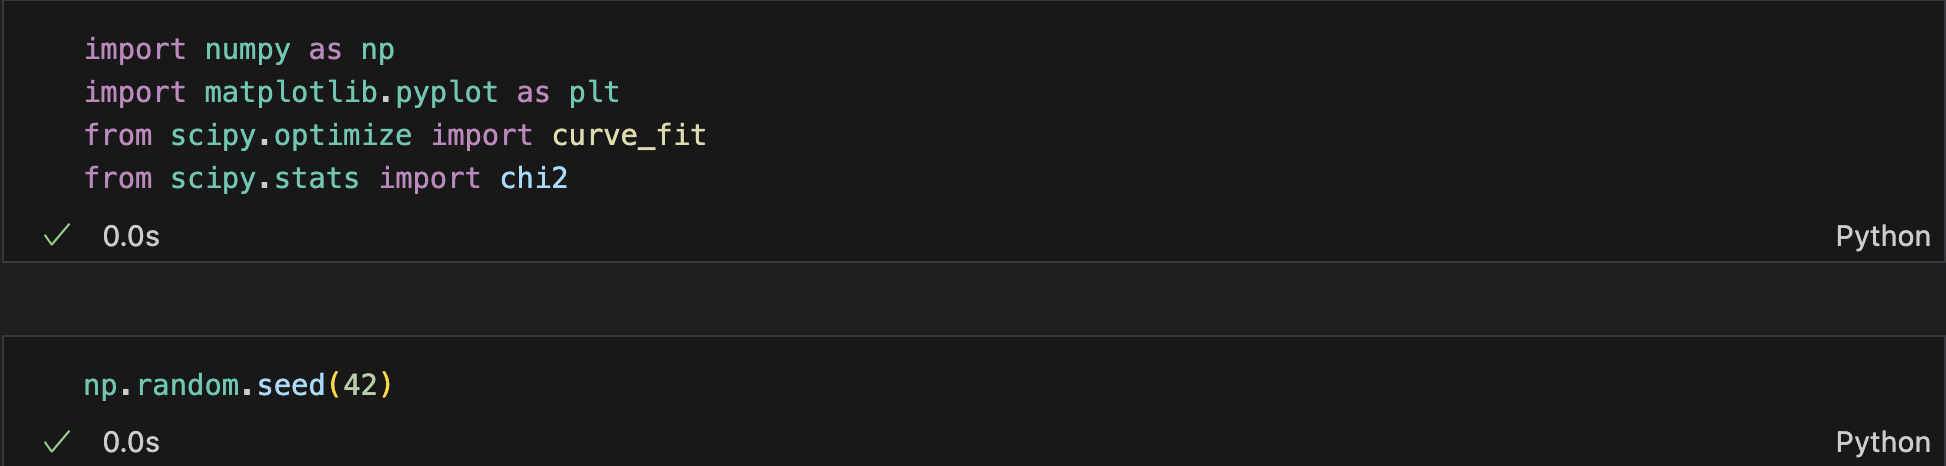
\includegraphics[width=1\linewidth]{figures/code/practice_1/code_1_1.png}
        \caption{Import packages and fix the random seed to 42}
        \label{fig:code_1_1}
    \end{figure}
    \item Generate \textcolor{red}{2000 sets} of data points defined by a function $y = a \ast x + b + \text{noise}$ with $x = \texttt{np.linspace}(1, 10, 10)$.
    
    \item The noise is sampled from a normal distribution with \textcolor{red}{mean = 0} and \textcolor{red}{standard deviation = $\sigma_0 = 3$}.

    \begin{figure}[h]
        \centering
        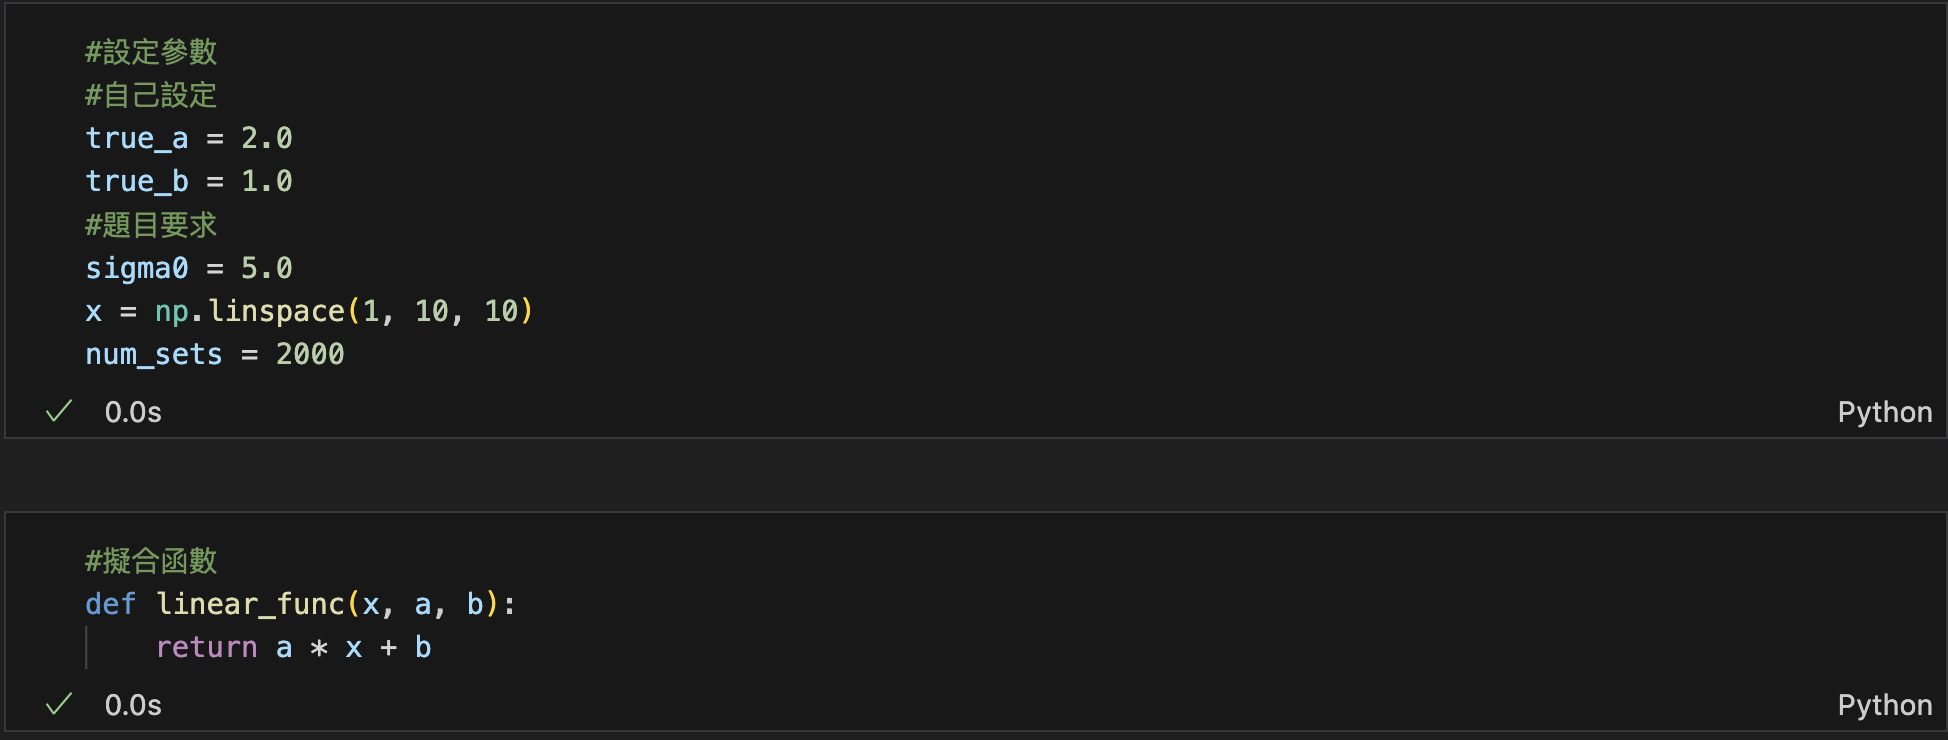
\includegraphics[width=1\linewidth]{figures/code/practice_1/code_1_2.png}
        \caption{Generate samples with assigned mean, noise, and dataset size.}
        \label{fig:code_1_2}
    \end{figure}
    
    
    \item Fit the data points \textcolor{red}{set by set} with the function $y = a \ast x + b$ using \texttt{curve\_fit}.
    
    \item Now calculate the $\chi^2$ for each set of data points. The standard deviation $\sigma_j$ may vary slightly but remains close to $\sigma_0$.
    
    \item $\chi^2_i = \sum_{j=1}^{10} \frac{(\text{data\_point}_{i,j} - \text{fitted\_result}_{i,j})^2}{\sigma_j^2} \quad (i = 1 \sim 2000)$
    where $i$ is the index of data set and $j$ is the index of $x$ value in one data set. (len($\chi^2$) = 2000)
    
    \item You might find out that this $\chi^2$ is just the sum of the squares of the residuals divided by the standard deviation, and it is analogous to previous practice: summing up the $\chi^2$ of each normal distribution sample.

    \begin{figure}[h]
        \centering
        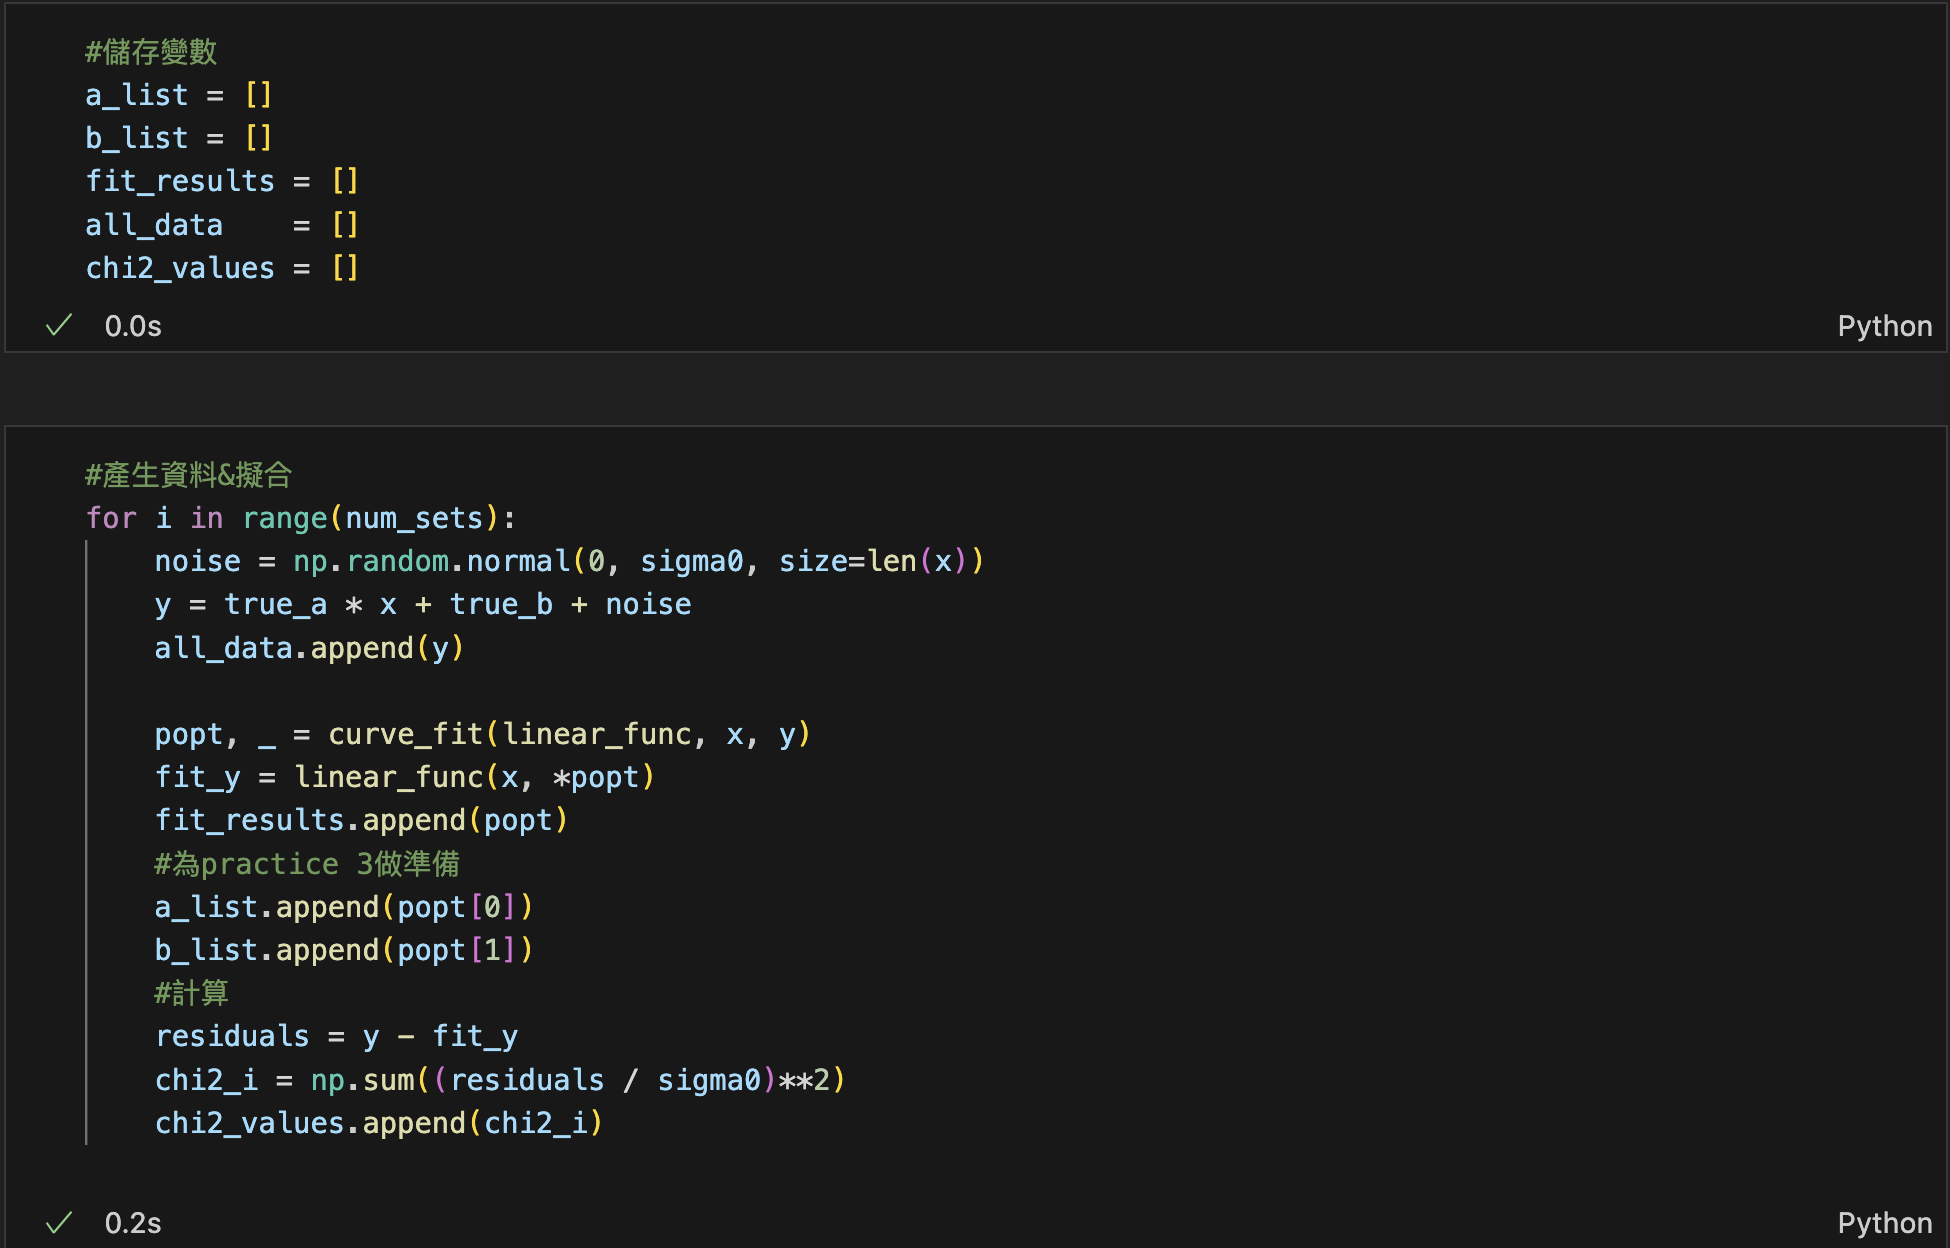
\includegraphics[width=1\linewidth]{figures/code/practice_1/code_1_3.png}
        \caption{Fit the data points set by set and calculate the $\chi^2$ values.}
        \label{fig:code_1_3}
    \end{figure}

    % \clearpage
    \item Plot all data points you have generated by $y = a \ast x + b + \text{noise}$.
    \begin{figure}[h]
        \centering
        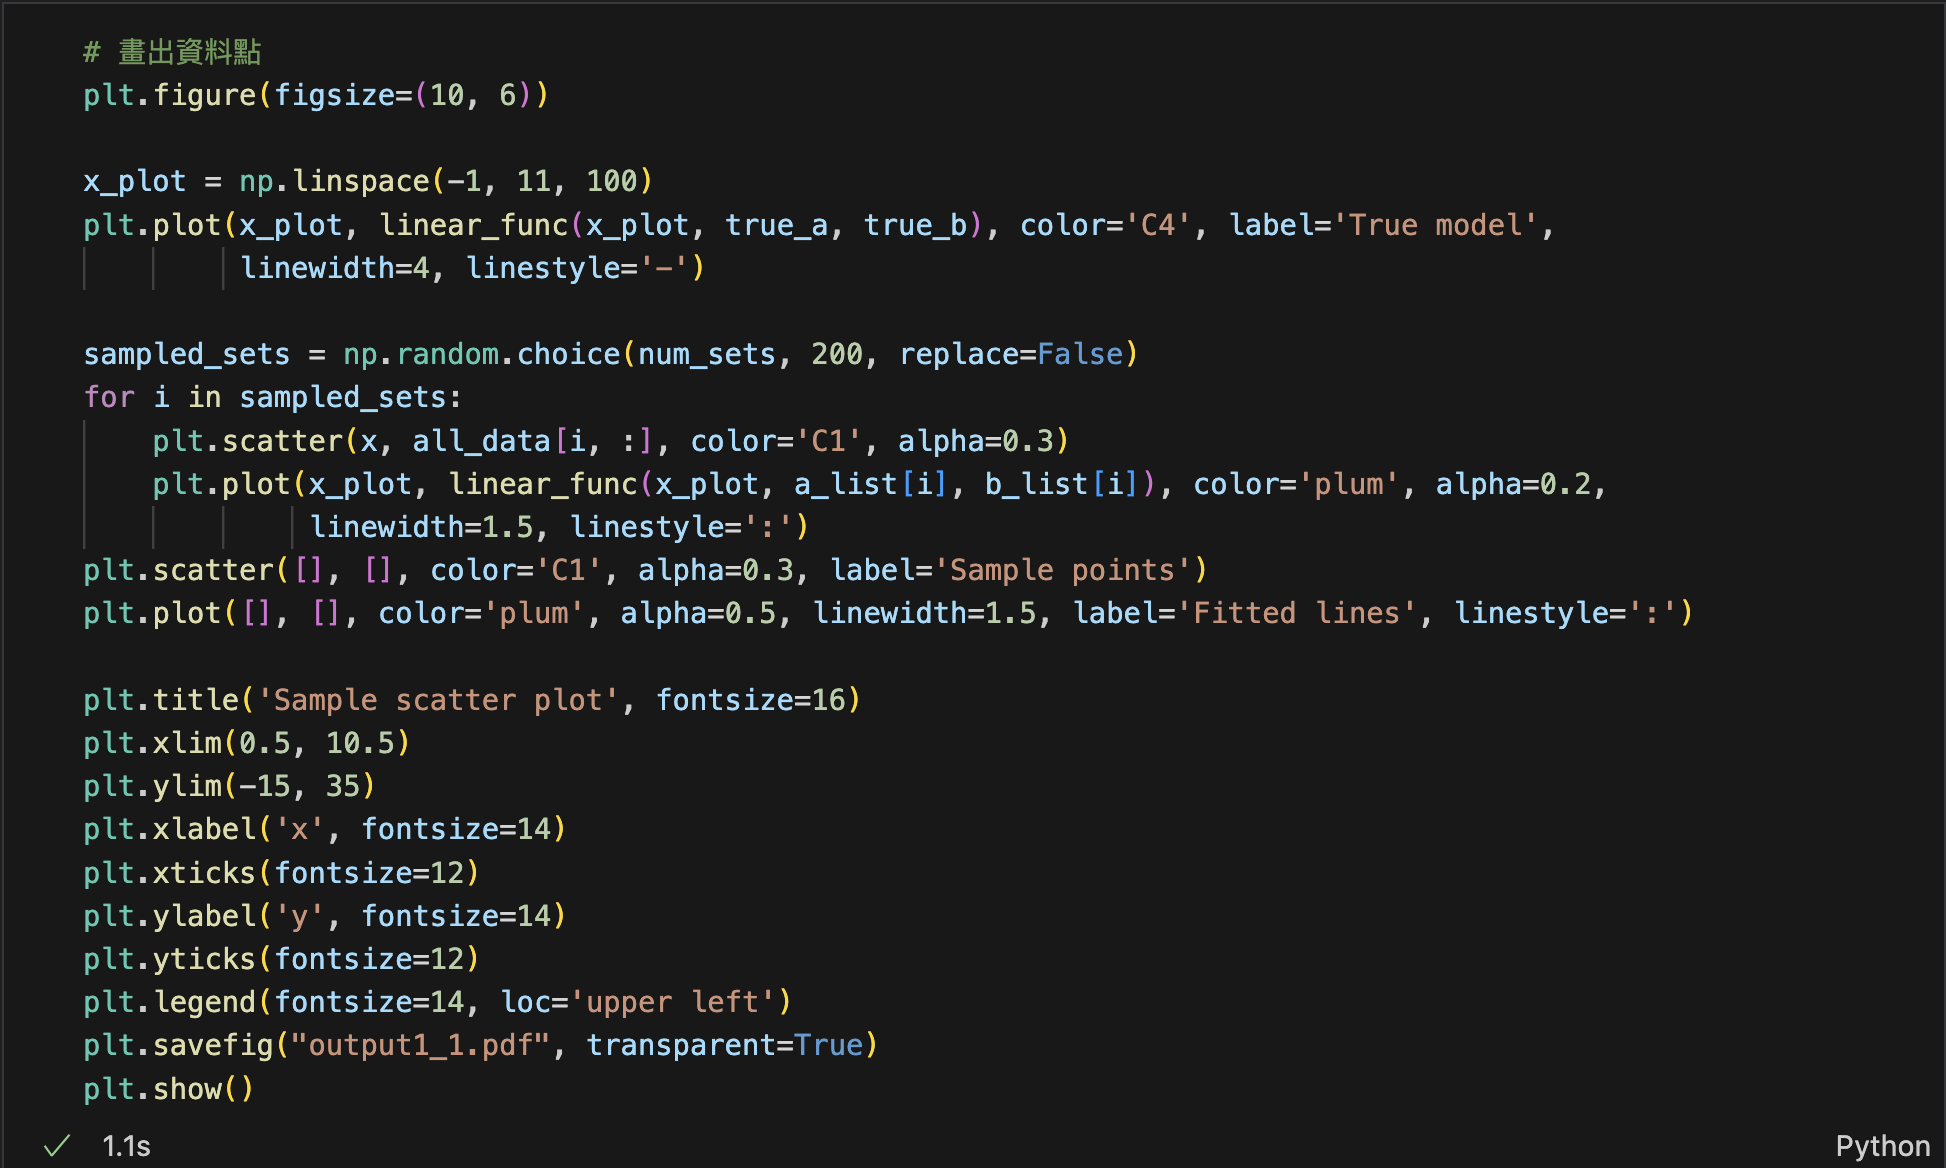
\includegraphics[width=1\linewidth]{figures/code/practice_1/code_1_4.png}
        \caption{Plot all data points}
        \label{fig:code_1_4}
    \end{figure}

    \clearpage
    \item Plot the histogram of these $\chi^2$ obtained from each set of data points. (A set of data points is a 10 points line with noise)
    
    \item Compare the histogram with the \textcolor{blue}{chi-square distribution}.
    \begin{figure}[h]
        \centering
        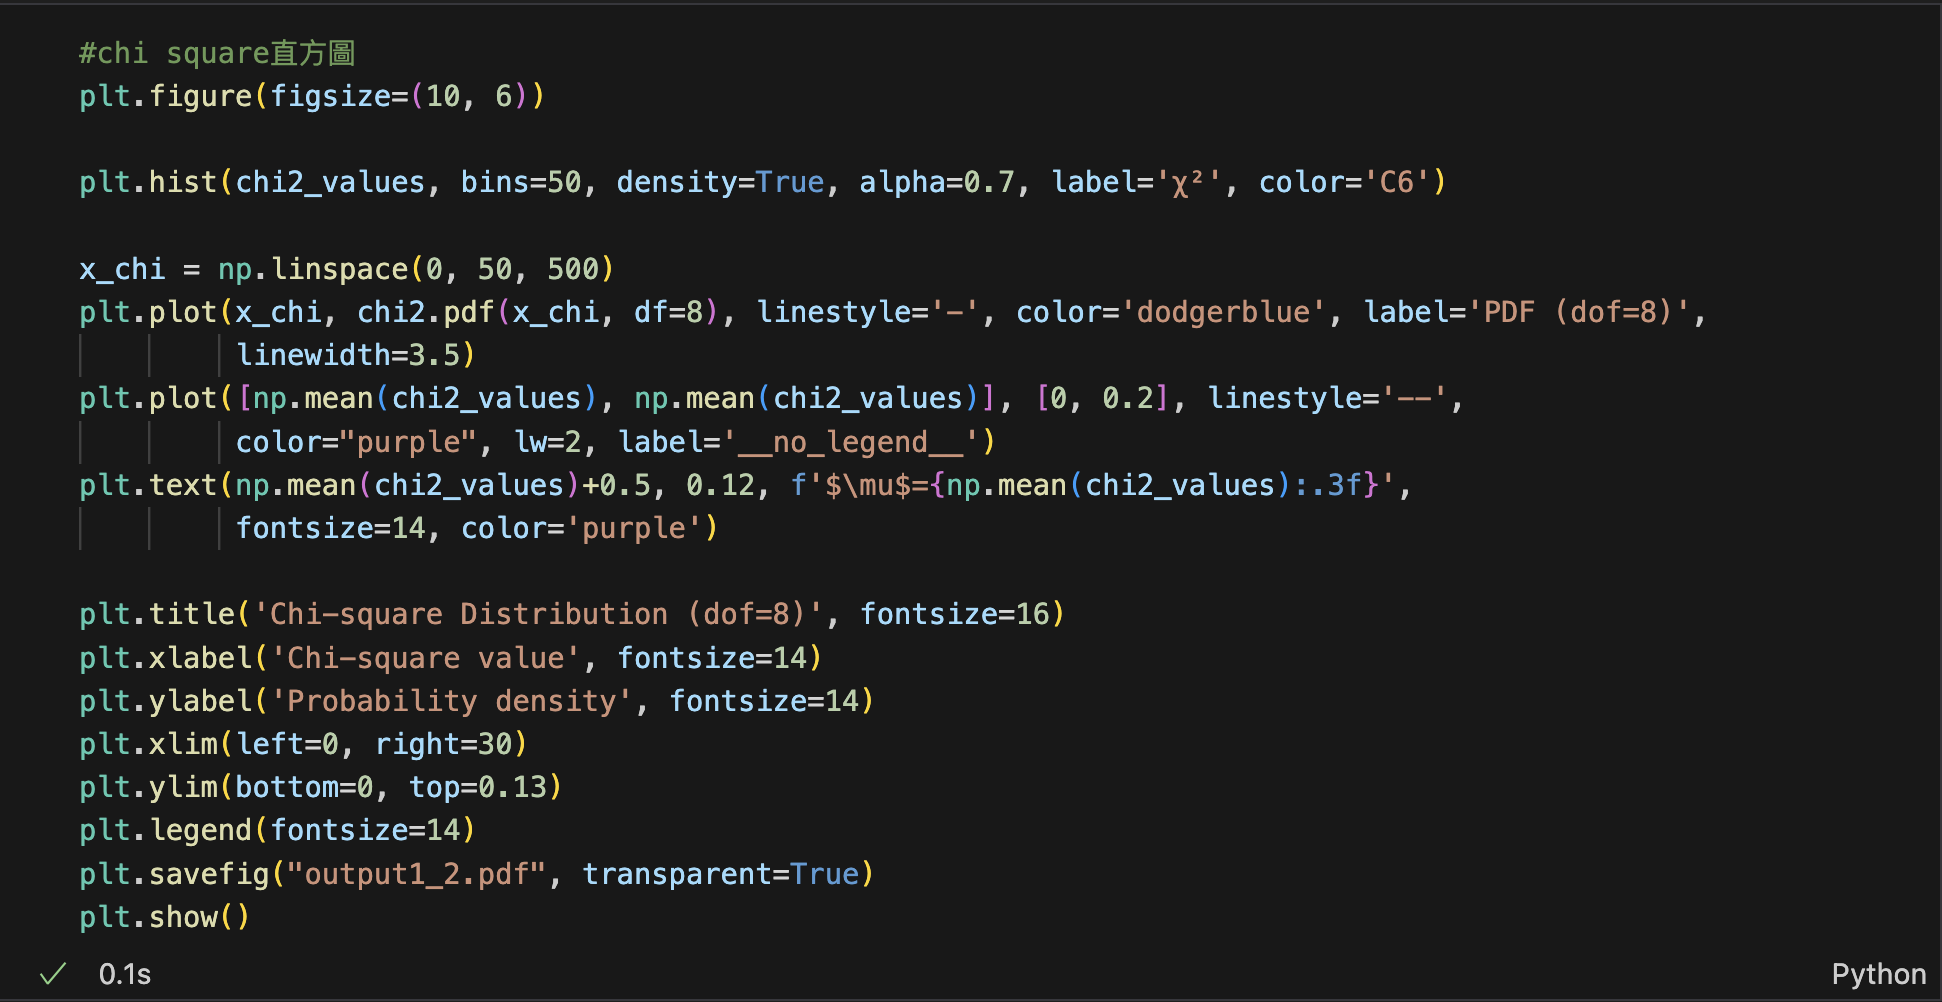
\includegraphics[width=1\linewidth]{figures/code/practice_1/code_1_5.png}
        \caption{Plot the histogram of the $\chi^2$ values and compare to the PDF of chi-square distribution}
        \label{fig:code_1_5}
    \end{figure}
    
\end{enumerate}

\clearpage
\subsection{Practice 2}
\hfill



\begin{enumerate}
    \item Show the histogram of $a$ and $b$ in \textbf{Practice 1} fitted in separated five sections shown in Figure 1.
    \begin{figure}[h]
        \centering
        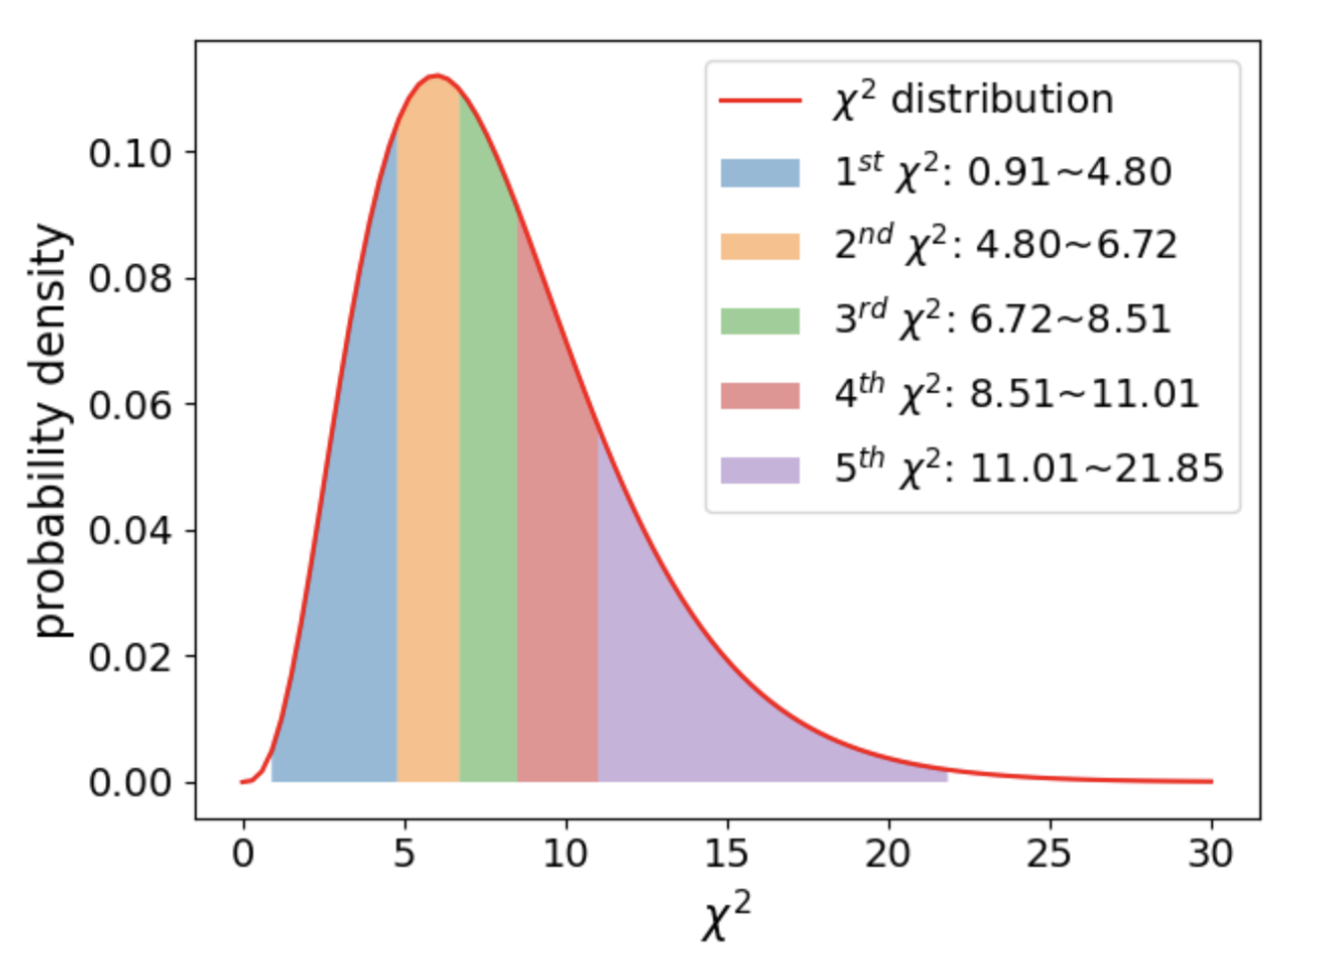
\includegraphics[width=0.85\linewidth]{figures/code/practice_2/fig1.png}
        \caption{"Figure 1" in the course material.}
        \label{fig:fig1}
    \end{figure}
    
    \item Each section contains \textcolor{red}{400 sets} of data points, grouped as follows: 1--400, 401--800, 801--1200, 1201--1600, and 1601--2000, ordered by $\chi^2$ value.
    
    \item You'll need to get those $a$ and $b$ values sorted by the $\chi^2$ value and choose certain indexes that are in the section to plot the histogram.
    \begin{figure}[h]
      \centering
      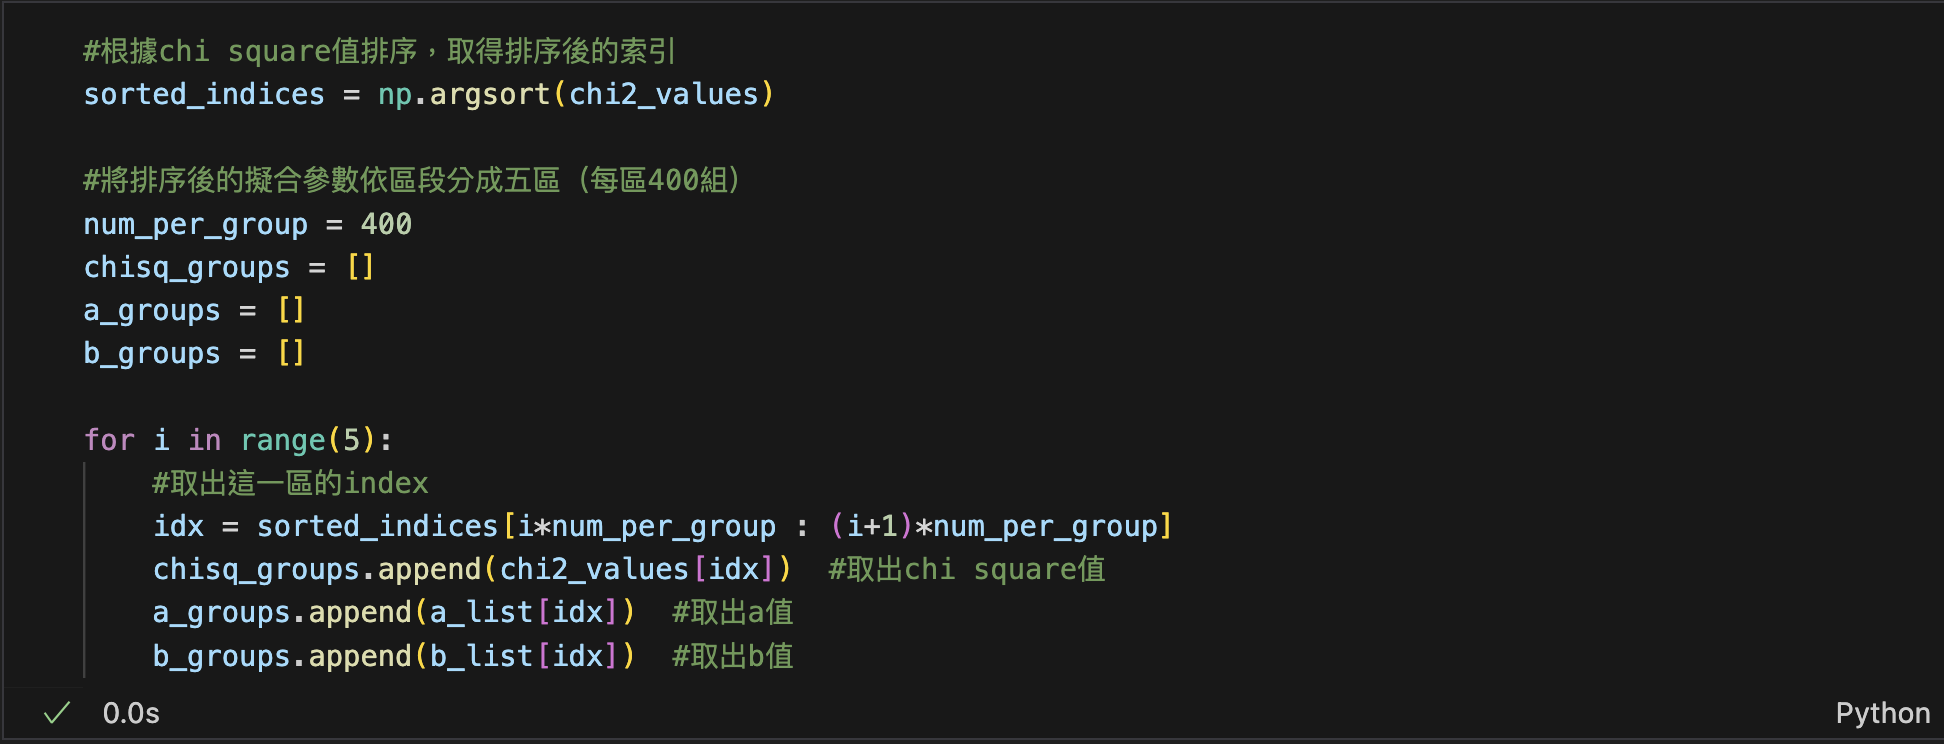
\includegraphics[width=1\linewidth]{figures/code/practice_2/code_2_1.png}
      \caption{Group data points into 5 groups according to their chi-square value}
      \label{fig:code_2_1}
    \end{figure}
    \begin{figure}[h]
      \centering
      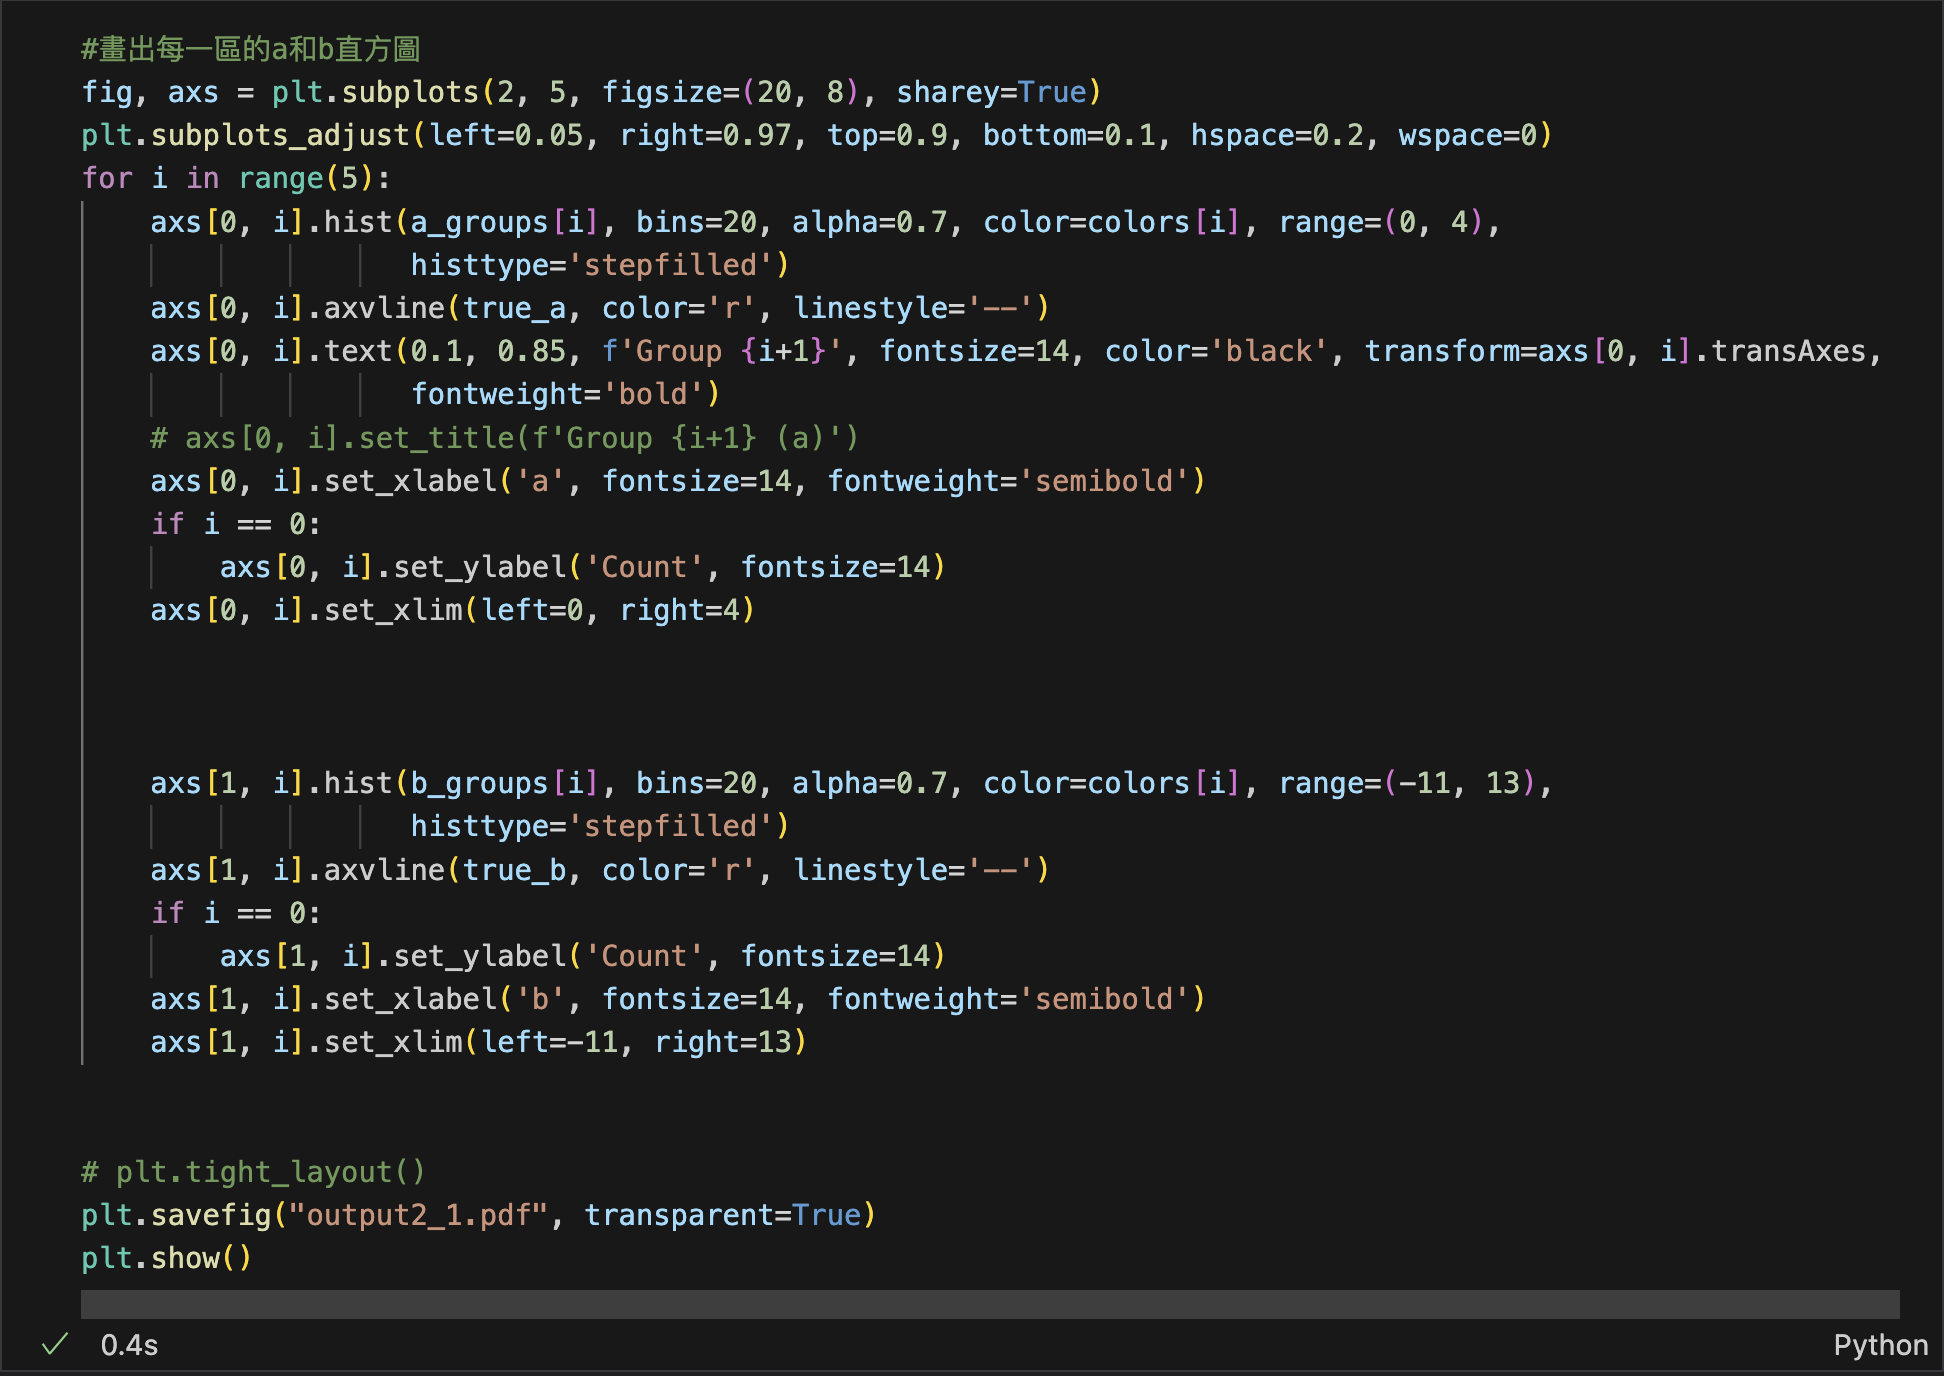
\includegraphics[width=1\linewidth]{figures/code/practice_2/code_2_2.png}
      \caption{Plot the histograms of $a$ and $b$ in five groups}
      \label{fig:code_2_2}
    \end{figure}
  
\end{enumerate}


\clearpage
\subsection{Practice 3}
\hfill


\begin{enumerate}
    \item By using the data points generated in \textbf{Practice 1}, get the mean and standard deviation of these data points.
    
    \item Fit these mean value of $y$ with the function \textcolor{red}{$y = a \ast x + b$} using \texttt{curve\_fit}, and remember to set \texttt{absolute\_sigma=True}.

    \begin{figure}[h]
        \centering
        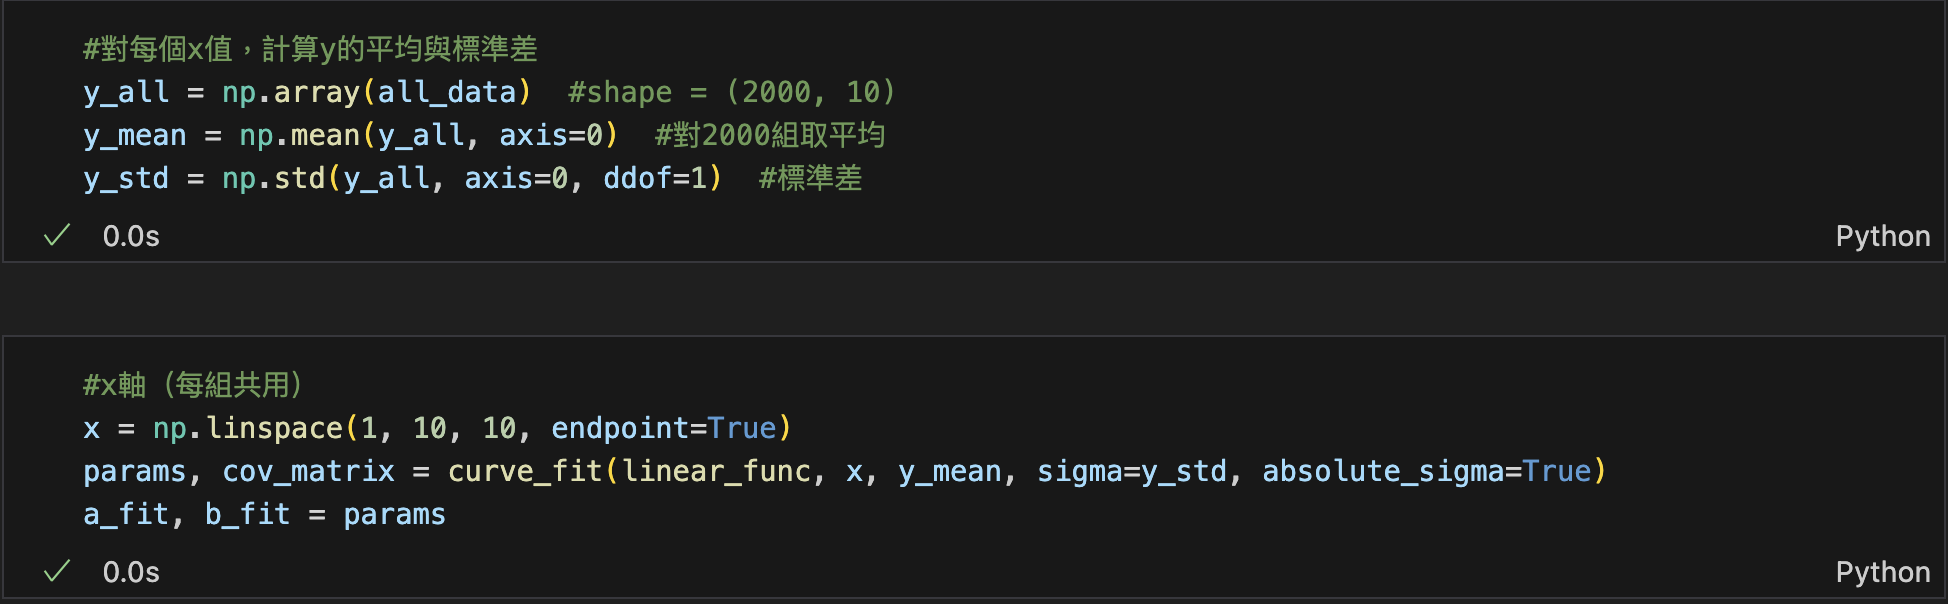
\includegraphics[width=1\linewidth]{figures/code/practice_3/code_3_1.png}
        \caption{Calculate the mean and standard deviation of the data points and fit them with \texttt{curve\_fit}}
        \label{fig:code_3_1}
    \end{figure}
    
    \item By using the result in \textbf{Practice 1}, you can show the histogram of those $a$ and $b$ values via \texttt{plt.hist} and \texttt{plt.hist2d} methods. (2000 sets of data points)

    \begin{figure}[h]
        \centering
        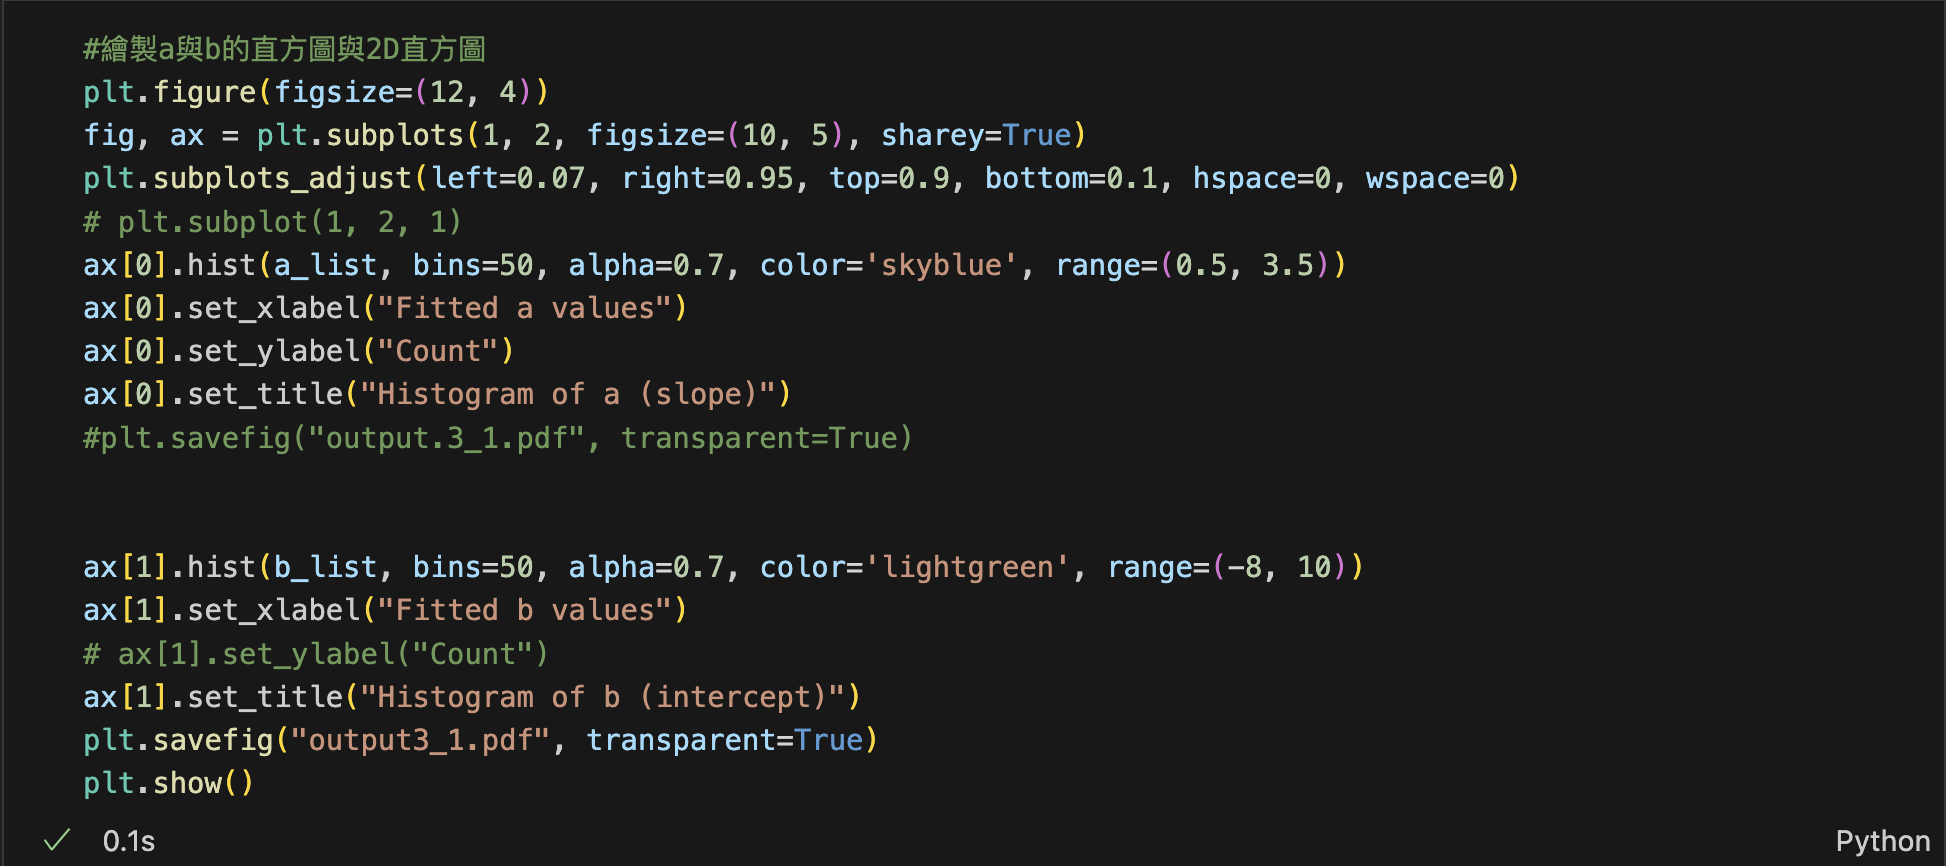
\includegraphics[width=1\linewidth]{figures/code/practice_3/code_3_2.png}
        \caption{1D histogram of the fitted results}
        \label{fig:code_3_2}
    \end{figure}
    \clearpage
    \begin{figure}[h]
        \centering
        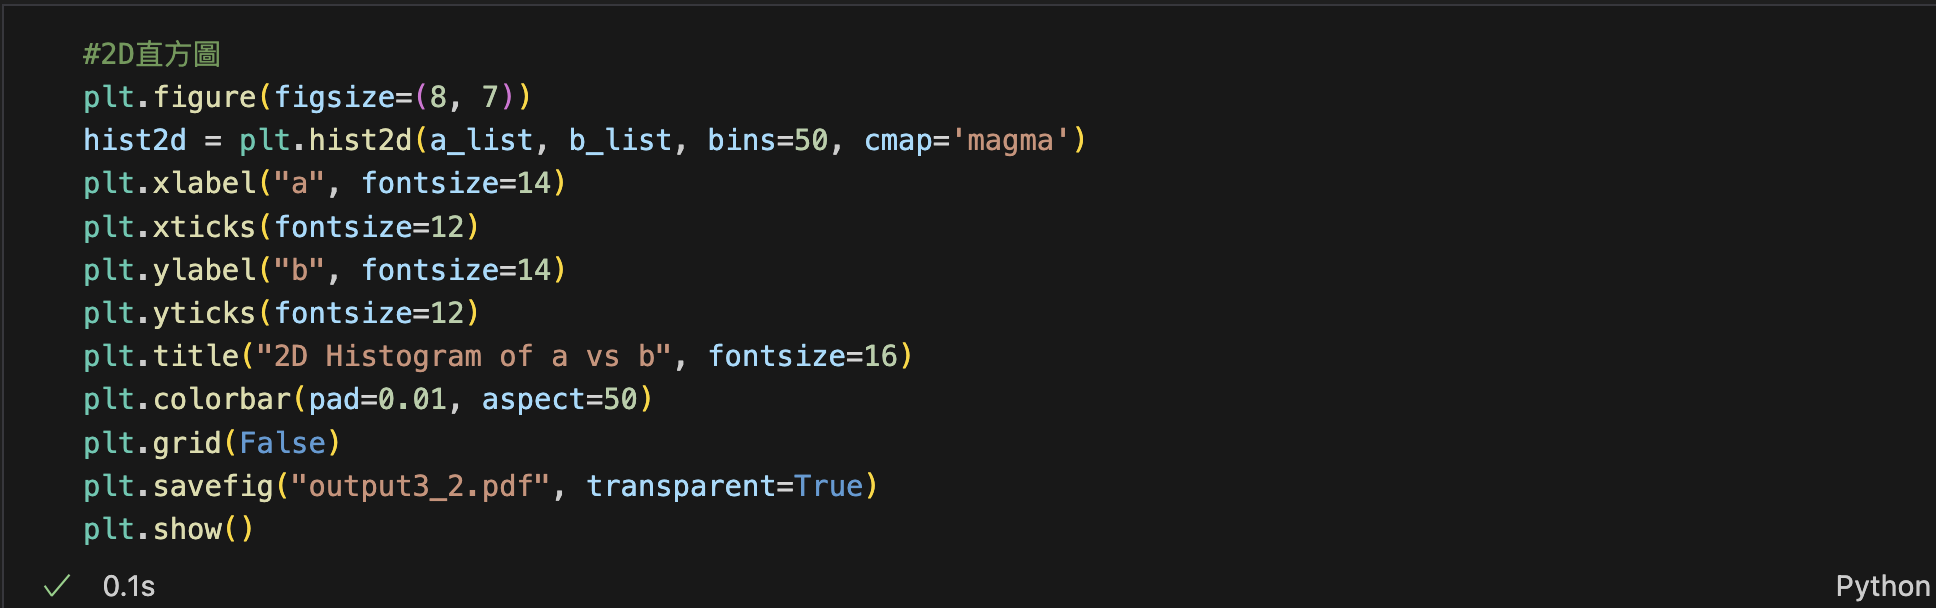
\includegraphics[width=1\linewidth]{figures/code/practice_3/code_3_3.png}
        \caption{2D histogram of the fitted results}
        \label{fig:code_3_3}
    \end{figure}
    
    % \clearpage
    \item Compare the standard deviation and correlation coefficient obtained from the \uline{fitted covariance matrix} with those derived from \uline{statistical graphs of $a$ and $b$}.
    
    \item Perform a linear fit on the 2D histogram of parameters $a$ and $b$ to obtain the slope, which characterizes certain properties useful for calculating the correlation coefficient.
    
    \item Ensure the definition of those quantities you are calculating is correct.
    
    \item Finally, you should be able to find that everything is consistent with the covariance matrix. (The values will be close to each other)
    \begin{figure}[h]
        \centering
        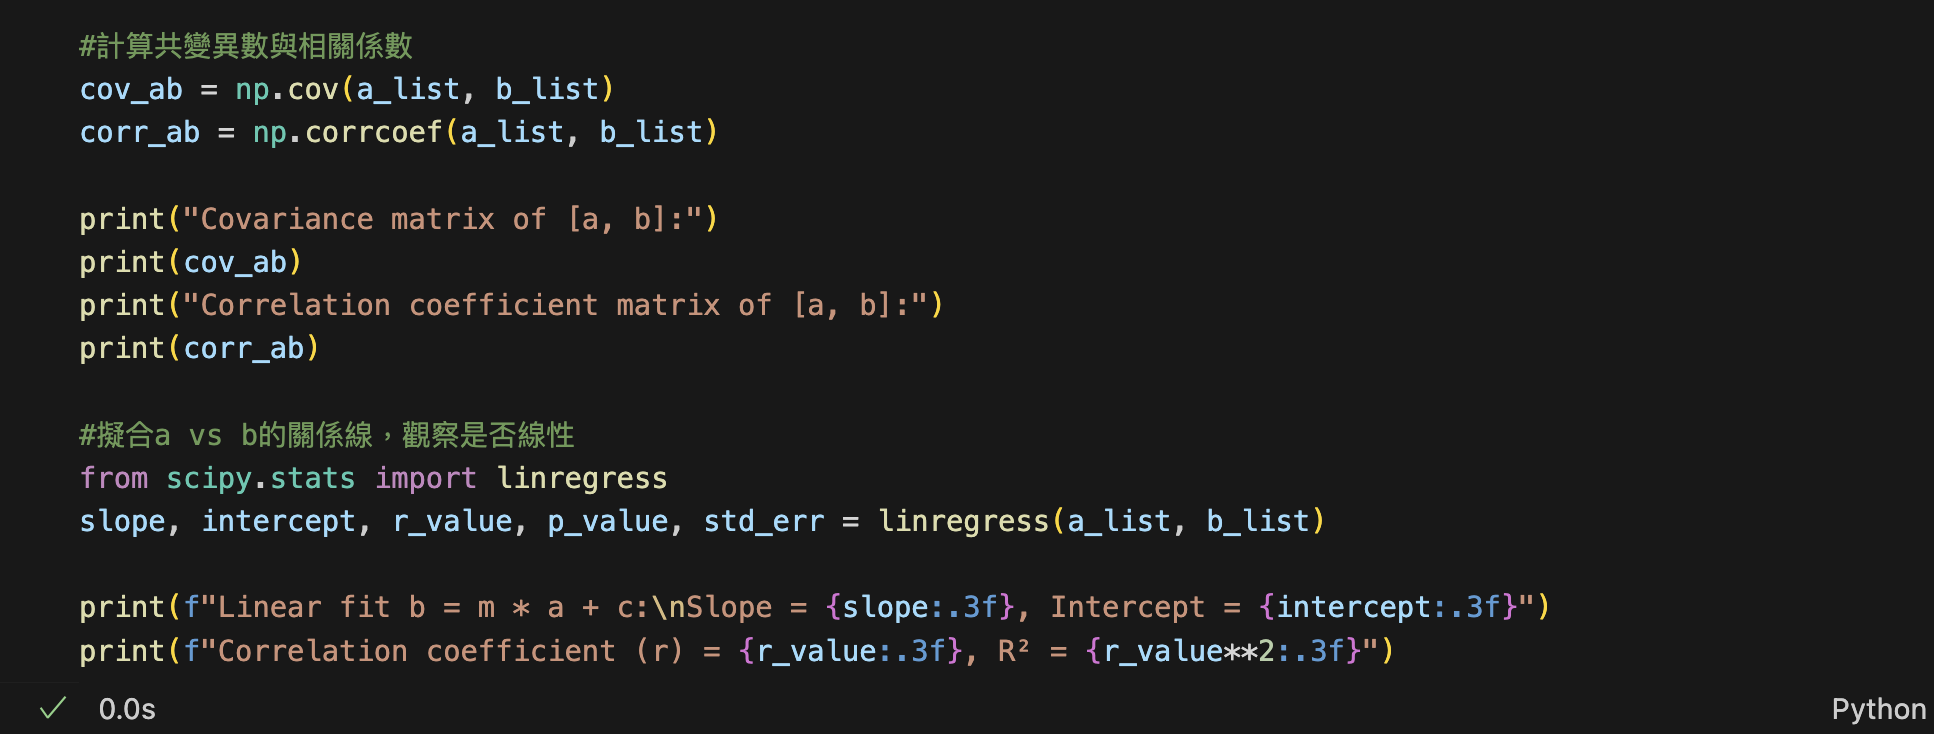
\includegraphics[width=1\linewidth]{figures/code/practice_3/code_3_4.png}
        \caption{Calculating the correlation coefficient by performing a linear fit on parameters $a$ and $b$}
        \label{fig:code_3_4}
    \end{figure}    
\end{enumerate}


\clearpage
\section{實驗數據與分析}
% \hfill

\subsection{Practice 1}\label{subsec:result_1}
\hfill

\begin{figure}[h]
    \centering
    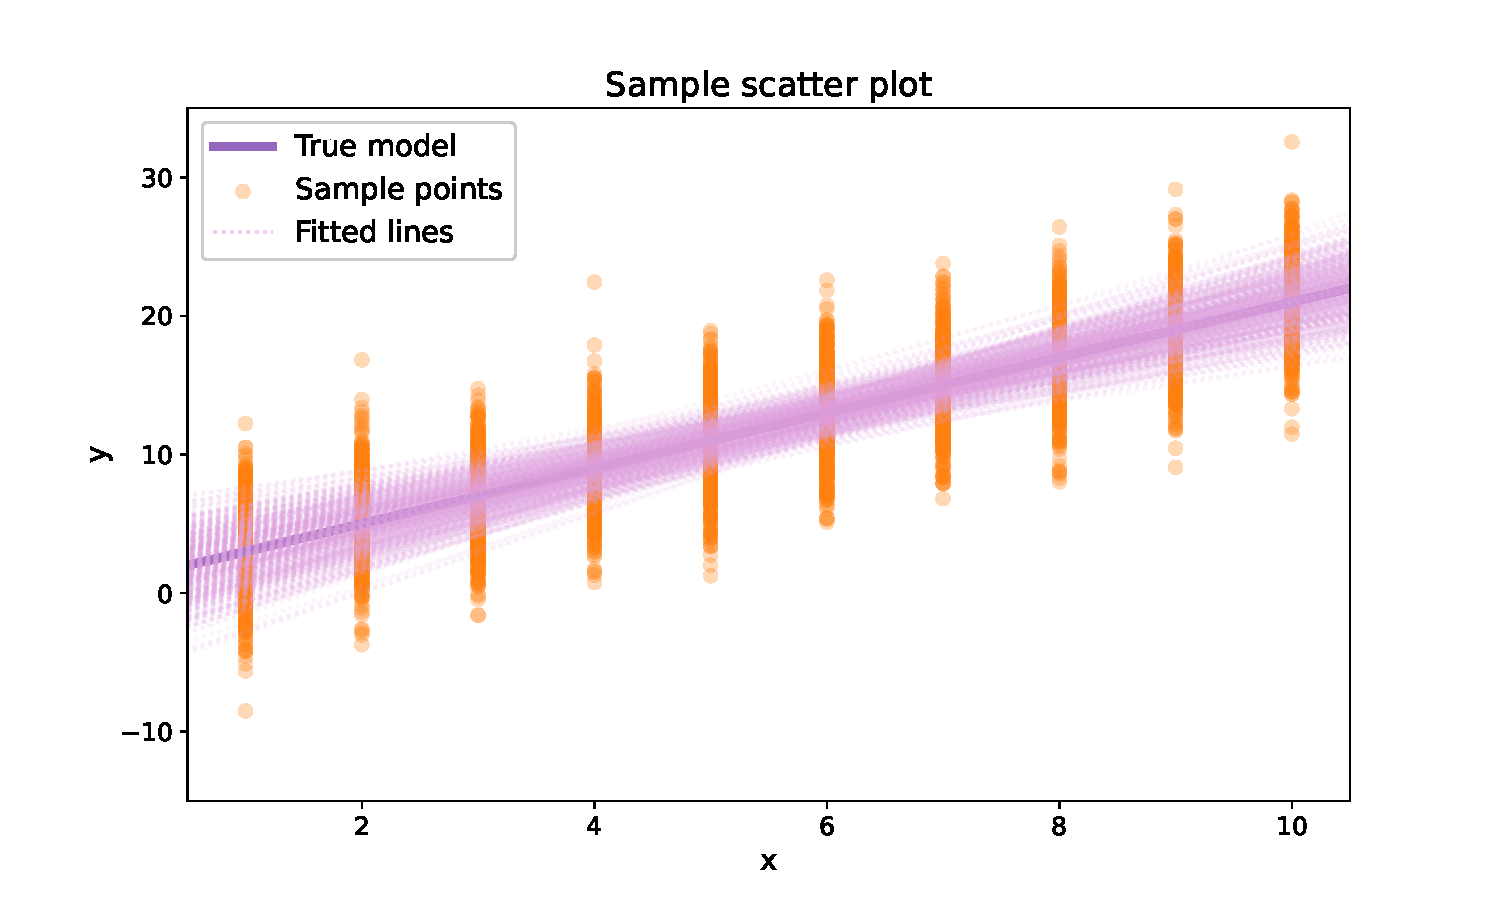
\includegraphics[width=.8\linewidth]{figures/output/practice_1/output1_1.pdf}
    \caption{Sample points of our data (plotted only 500 sets for representative)}
    \label{fig:output_1_1}
\end{figure}

 
\begin{figure}[h]
    \centering
    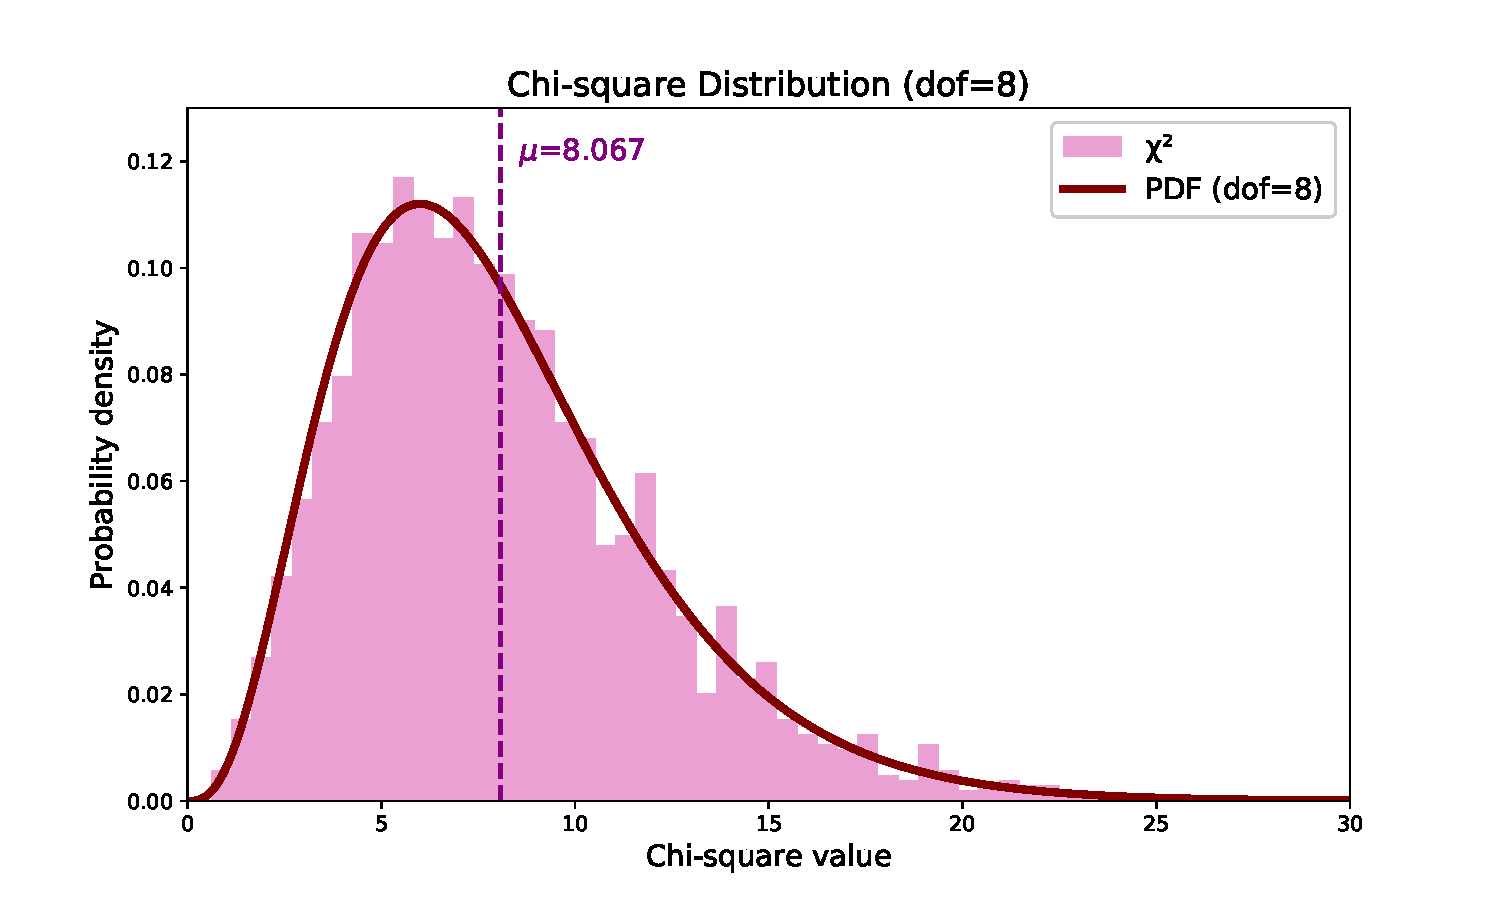
\includegraphics[width=.8\linewidth]{figures/output/practice_1/output1_2.pdf}
    \caption{Histogram of the chi-square distributions}
    \label{fig:output_1_2}
\end{figure}

Resembling last week's practices, the experimental dataset is sampled from a linear model $y=ax+b$ with a Gaussian noise $\sigma_0 = 3$. For clarification, Fig. \ref{fig:output_1_1} randomly plots 500 sets out of the 2000 datasets (orange scattered dots). The model and the fitted curves, generated by \texttt{curve\_fit} with the linear model, are also displayed in Fig. \ref{fig:output_1_1} (purple solid and dotted lines, respectively). The means and the standard deviations of the data are listed in the Table. \ref{tab:mean_std}. 

The histogram of chi-square values is shown in Fig. \ref{fig:output_1_2}, overlapped with the probability density function (PDF) of the chi-square distribution with degrees of freedom (dof) equal to 8. The dof $\nu$ is assigned to be $ N-p = 10-2=8$ (Sec. \ref{subsec:goodness}). As expected, the mean chi-square value of 8.067 approximates the degrees of freedom, and the probability density function aligns well with the chi-square distribution.

% \clearpage
\subsection{Practice 2}
\hfill

%\hynote{The ideal result of this practice is that we can see the difference between each group on the $a$ and $b$ histograms: the distribution of the low-$\chi^2$ groups is more centrally concentrated, and vice versa. However, since the discrepancy of the chi-square values is not large enough, we can't get the proper result. (Or maybe our code is wrong.)}

\begin{figure}[h]
    \centering
    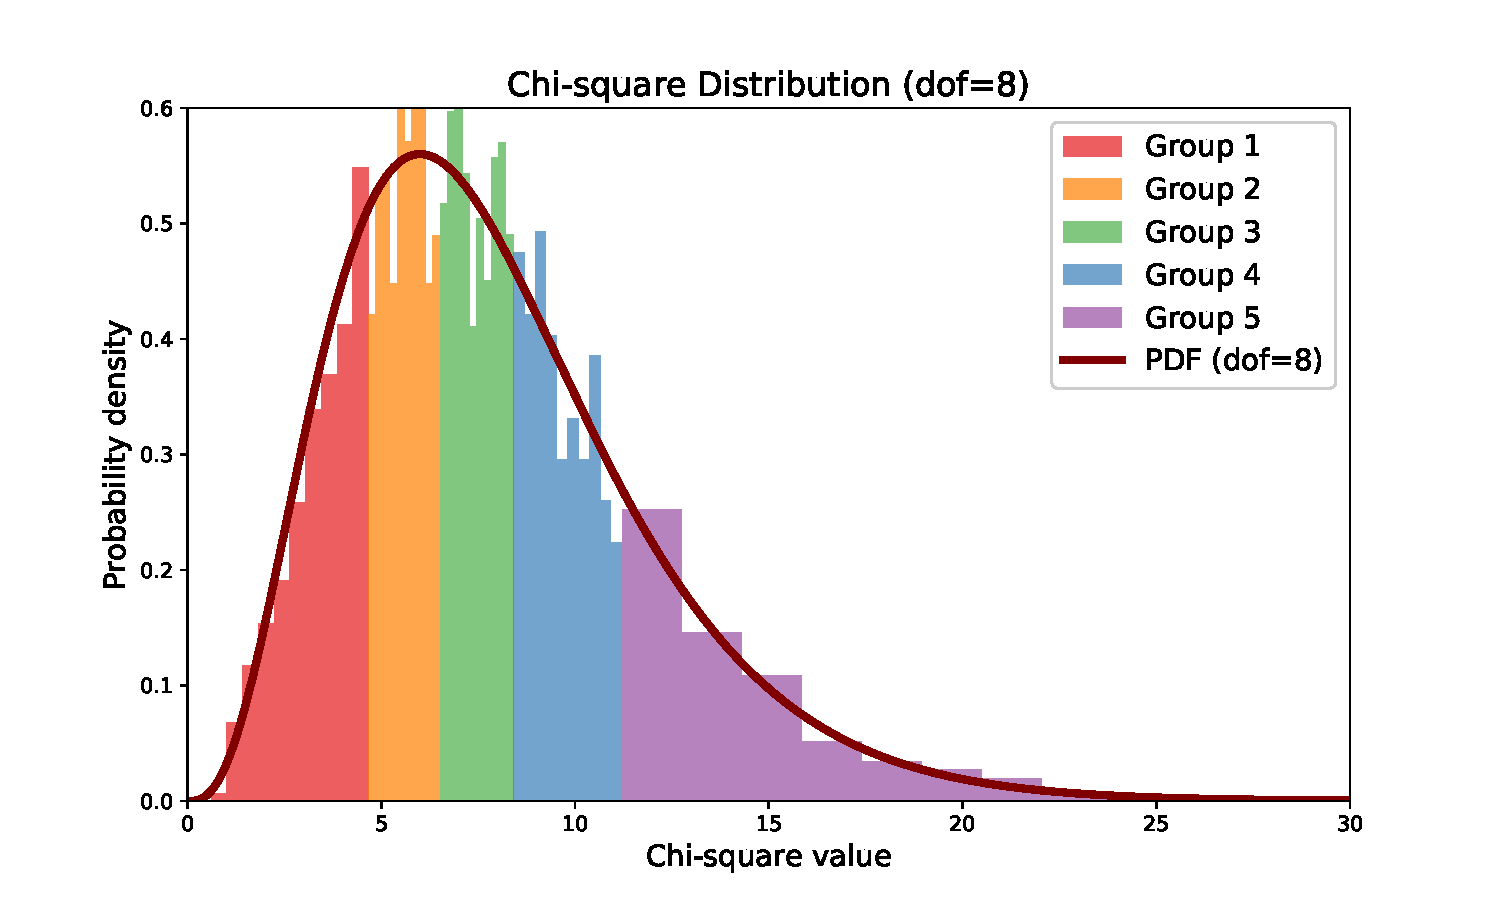
\includegraphics[width=.9\linewidth]{figures/output/practice_2/output2_1_chi_grouped.pdf}
    \caption{Chi-square distribution separated into five groups according to their chi-square values}
    \label{fig:output_2_1_chi_group}
\end{figure}

\begin{figure}[h]
    \centering
    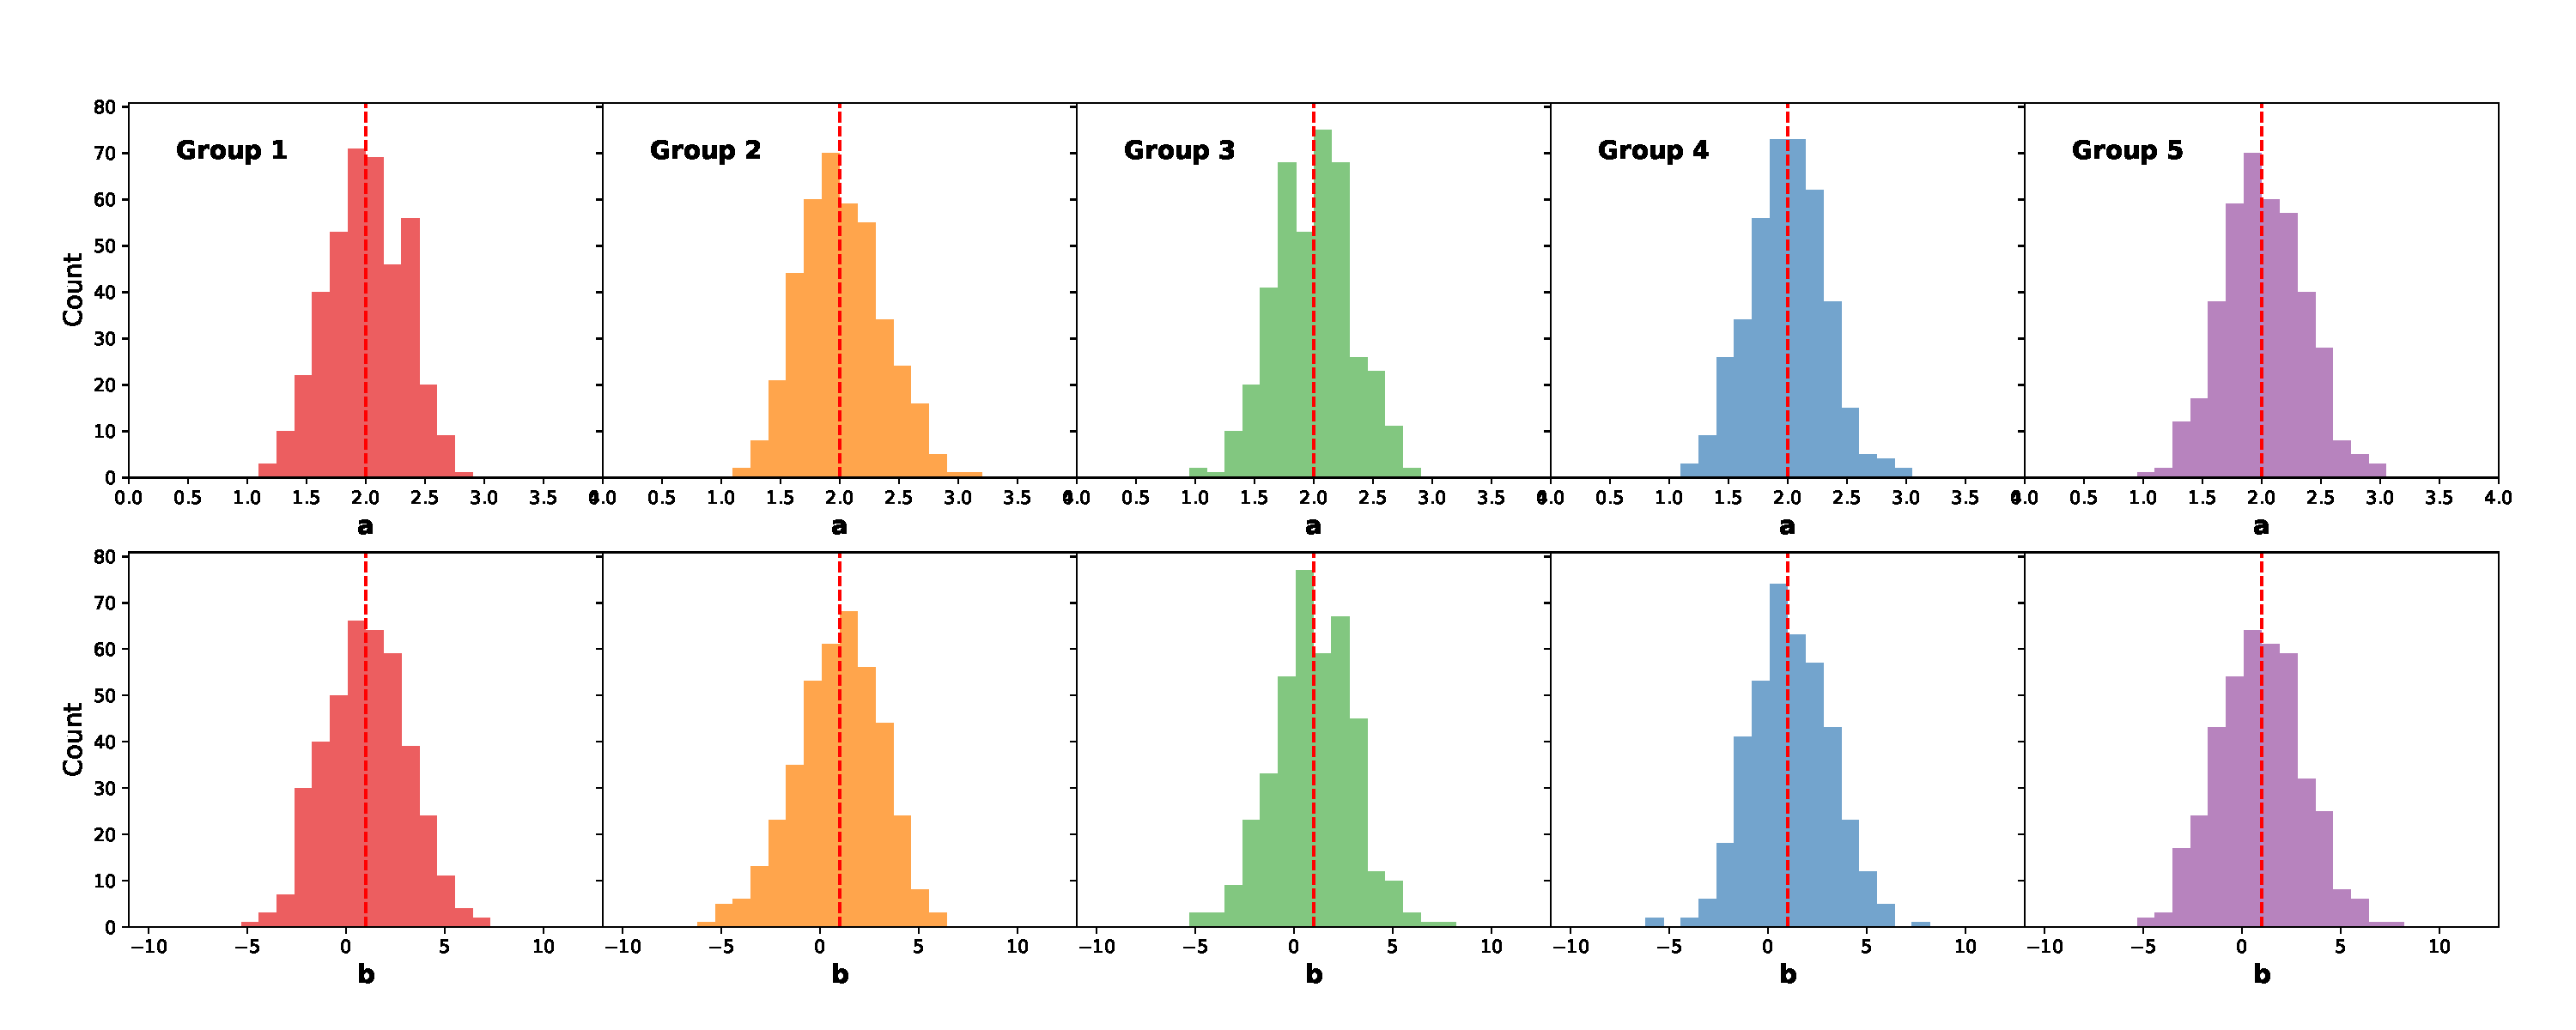
\includegraphics[width=1\linewidth]{figures/output/practice_2/output2_1.pdf}
    \caption{Histograms of $a$ and $b$}
    \label{fig:output_2_1}
\end{figure}
\clearpage
\begin{figure}[h]
    \centering
    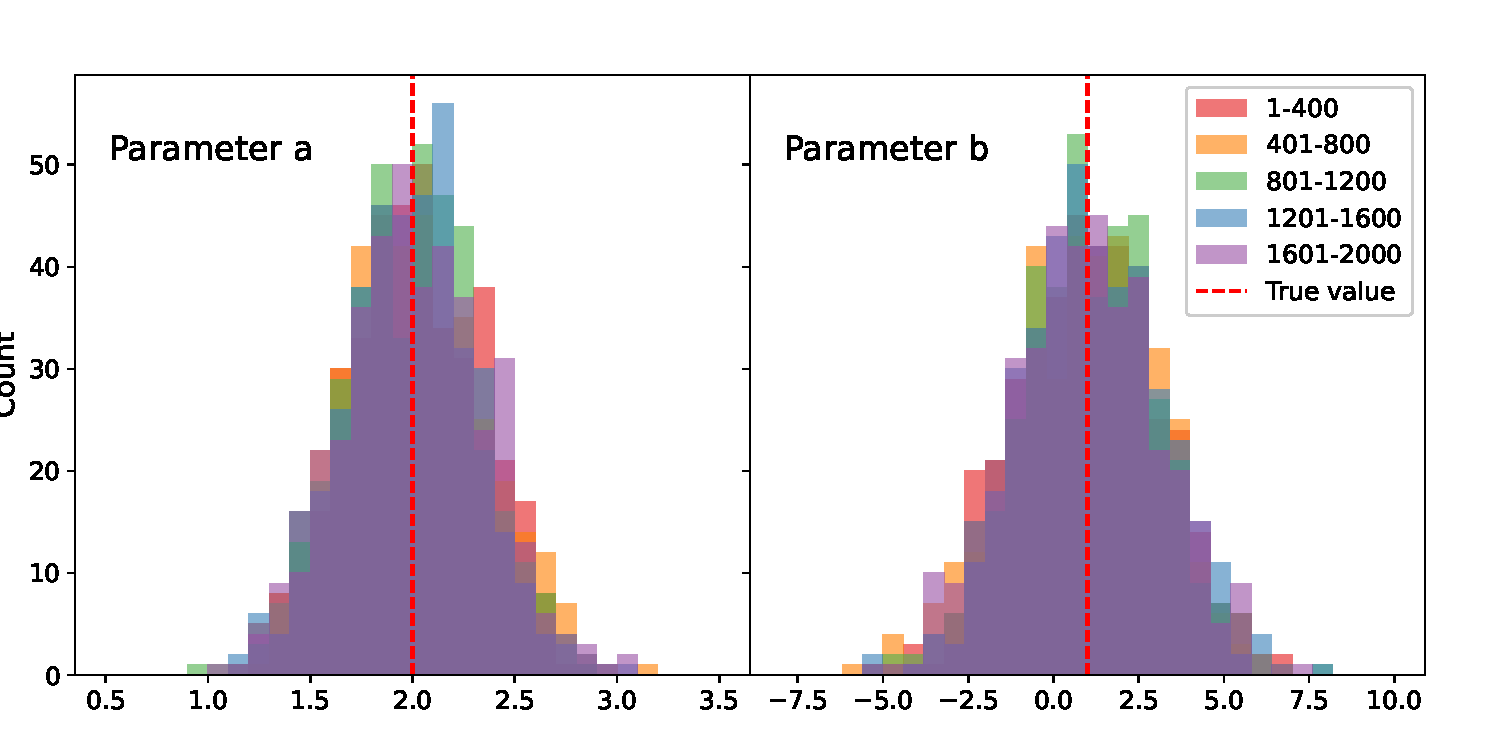
\includegraphics[width=1\linewidth]{figures/output/practice_2/output2_1_combine.pdf}
    \caption{Overlap the five histograms of Fig. \ref{fig:output_2_1}}
    \label{fig:output_2_1_combine}
\end{figure}

可從Fig.\ref{fig:output_2_1_chi_group} $\sim$ Fig.\ref{fig:output_2_1_combine}可見結果不合預期,分組差異不明顯。

分析原因如下:
\begin{itemize}
    \item 原本每組資料之標準差固定為3.0,導致資料的誤差相同,無法用$\chi^2$分辨擬合好壞。
    \item $\chi^2$之計算會將殘差標準化,所以每一組都使用對應的$\sigma$計算$\chi^2$,當誤差太大時,其會使公式分母變大,使$\chi^2$看起來還是很小。
\end{itemize}

我們透過以下方式改進:
\begin{itemize}
    \item 讓每組資料的標準差不同,提升數據的變異性。
    \begin{figure}[h]
        \centering
        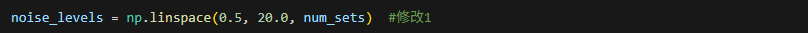
\includegraphics[width=1\linewidth]{figures/code/practice_2/practice_2_revise.png}
        \caption{修改後程式碼(1)}
        \label{fig:practice_2_revise1}
    \end{figure}
    \item 不使用$\chi^2$分組,改成使用$\sigma$分組。
    \begin{figure}[h]
        \centering
        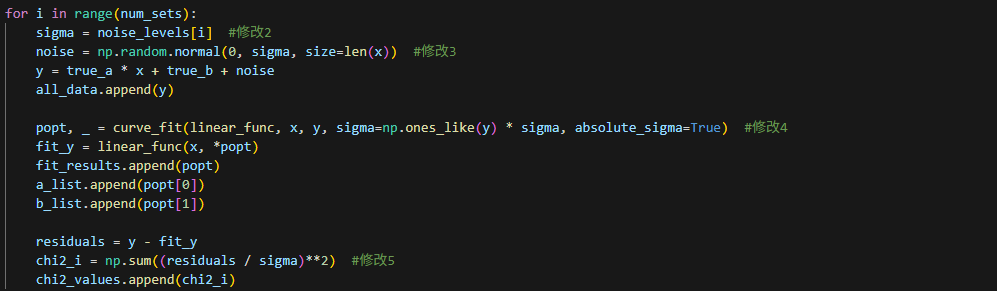
\includegraphics[width=1\linewidth]{figures/code/practice_2/practice_2_revise2.png}
        \caption{修改後程式碼(2)}
        \label{fig:practice_2_revise2}
    \end{figure}
    \clearpage
    \item 修改疊圖順序,使結果更明顯。
    \begin{figure}[h]
        \centering
        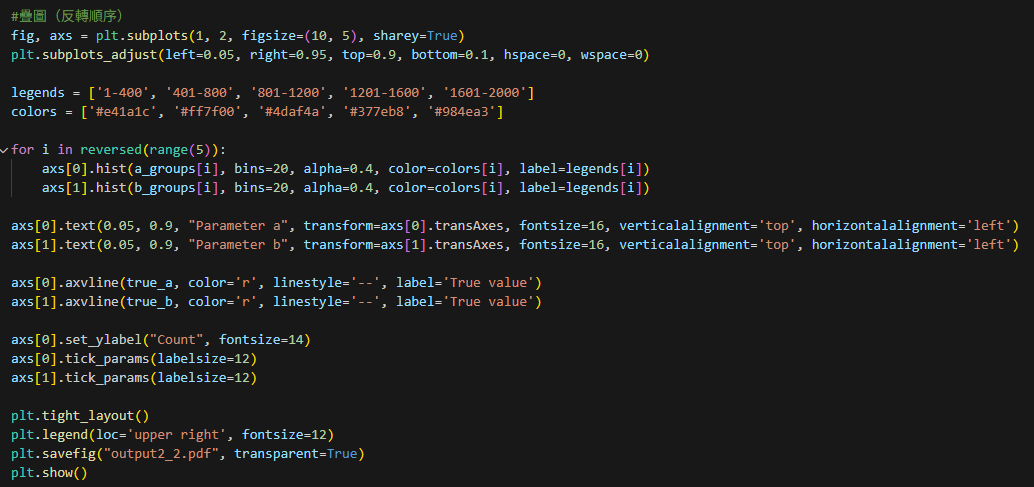
\includegraphics[width=1\linewidth]{figures/code/practice_2/practice_2_revise3.png}
        \caption{修改後程式碼(3)}
        \label{fig:practice_2_revise3}
    \end{figure}
    \clearpage
    修改後輸出結果如下:
\begin{figure}[h]
    \centering
    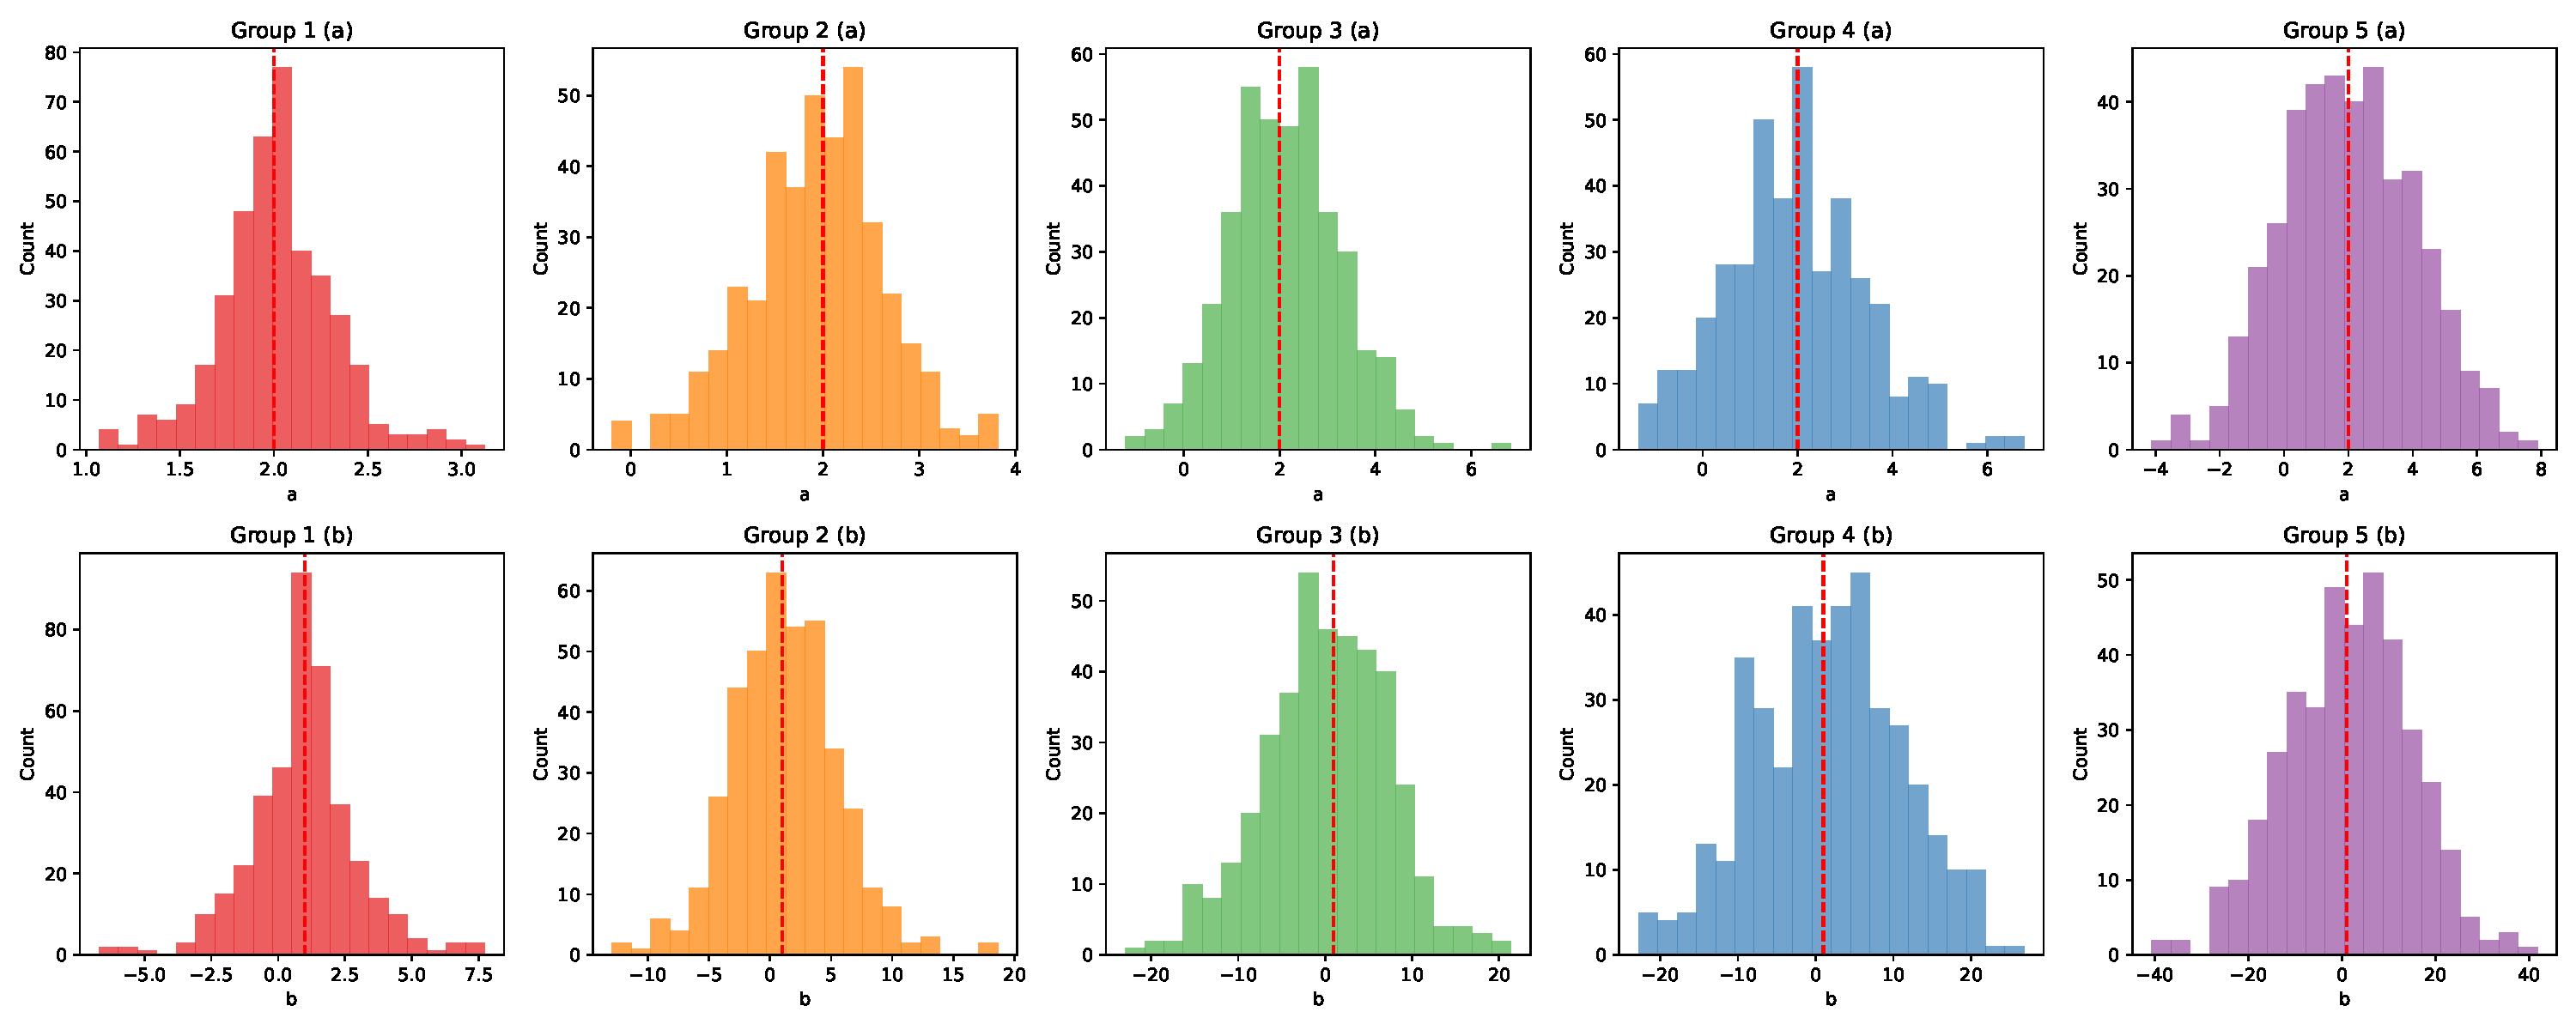
\includegraphics[width=1\linewidth]{figures/output/practice_2/output2_1_revise.pdf}
    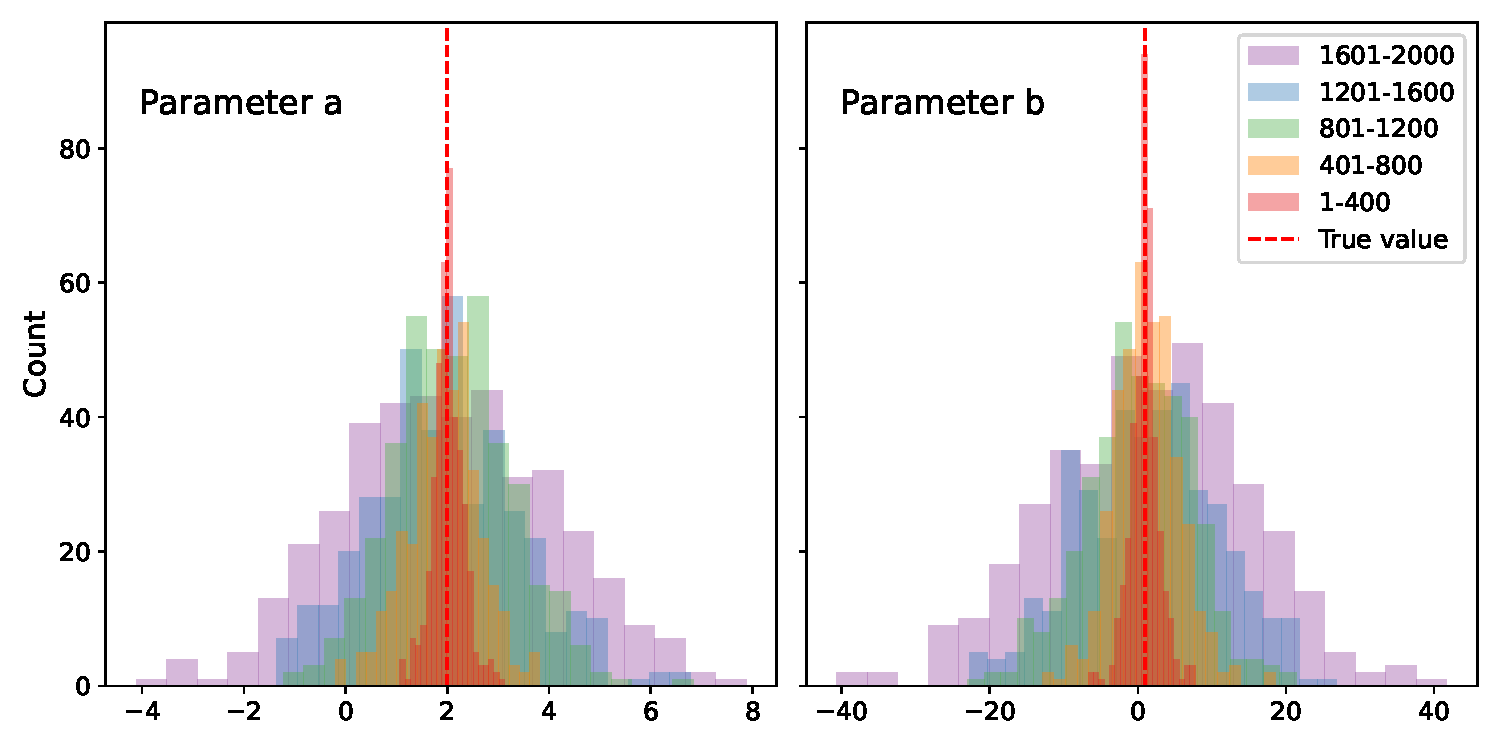
\includegraphics[width=1\linewidth]{figures/output/practice_2/output2_2_revise.pdf}
    \caption{修改後a和b的直方圖與其疊圖}
    \label{fig:practice_2_revise1}
\end{figure}
\end{itemize}

將數據根據誤差分成五組時,可觀察到擬合參數a與b的分布隨著誤差增大而變得分散。$Group\ 1$(誤差較低)分布最集中;$Group\ 5$(誤差較高)則分布較廣,成功呈現預期的趨勢。

\clearpage
\subsection{Practice 3}
\hfill

\begin{figure}[h]
    \centering
    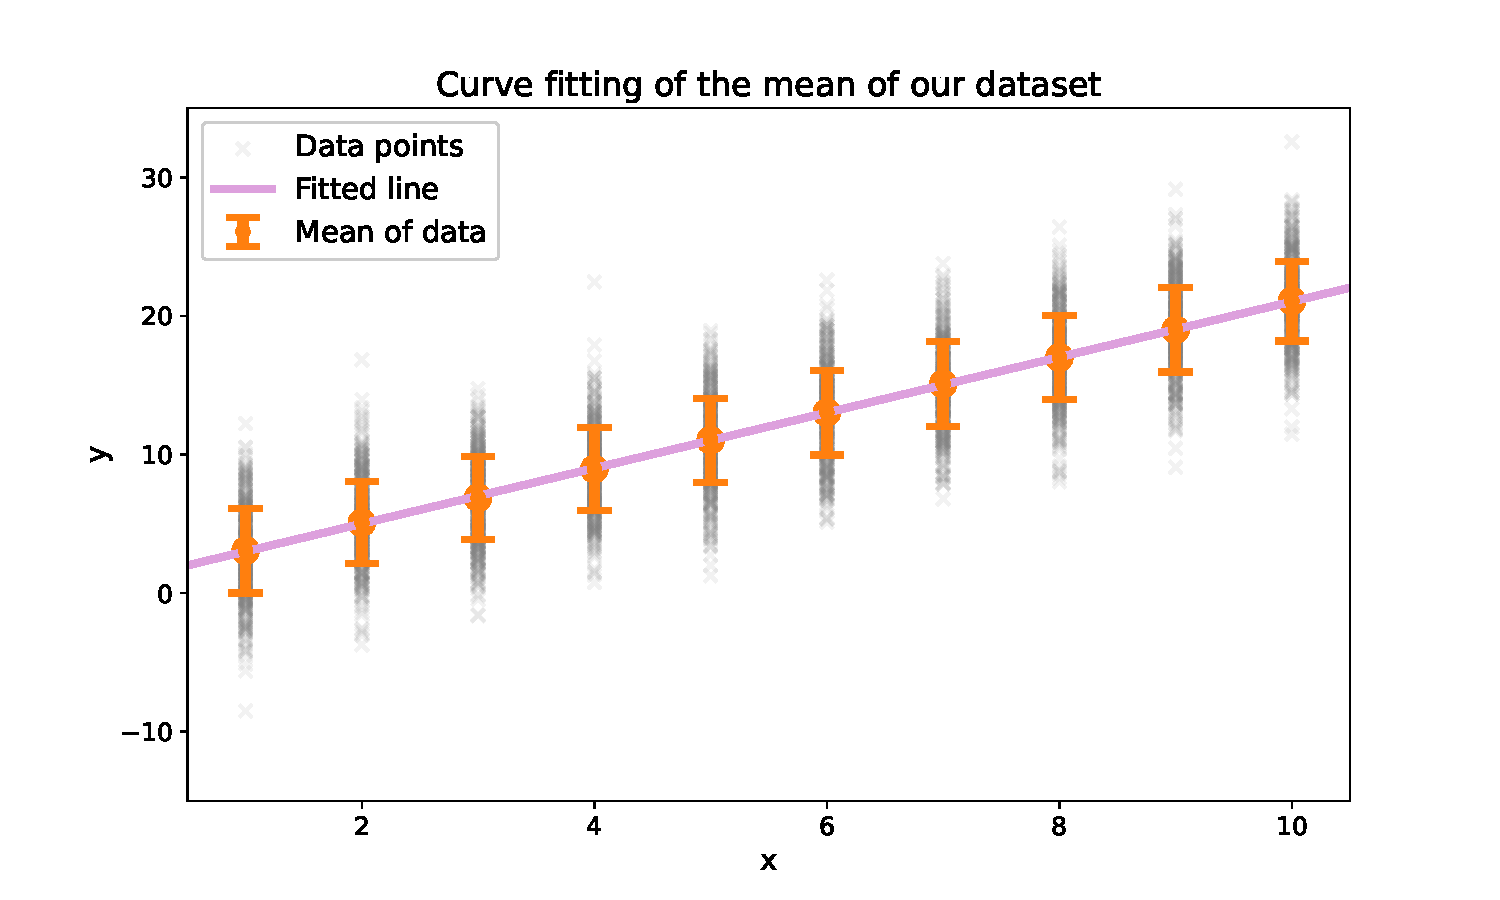
\includegraphics[width=1\linewidth]{figures/output/practice_3/output3_1.pdf}
    \caption{Curve fitting of the mean of the dataset (The fitted line is $y = 2.003x+1.002$)}
    \label{fig:output_3_1}
\end{figure}


\begin{table}[h]
\centering
\caption{The mean and standard deviation of data}
\label{tab:mean_std}
\vspace{.5cm}
\begin{tabular}{c||c c:c}
$x$ &   $y_{model}$ &   $\mu_{data}$  &   $\sigma_{data}$\\\hline\hline
1   &   3   &   3.07    &   3.06\\
2   &   5   &   5.08    &   2.97\\
3   &   7   &   6.88    &   3.00\\
4   &   9   &   8.95    &   2.97\\
5   &   11  &   11.03   &   3.03\\   
6   &   13  &   13.02   &   3.06\\
7   &   15  &   15.08   &   3.05\\   
8   &   17  &   16.99   &   3.02\\
9   &   19  &   19.00   &   3.04\\
10  &   21  &   21.07   &   2.88\\ 
\end{tabular}
\end{table}

\begin{figure}[h]
    \centering
    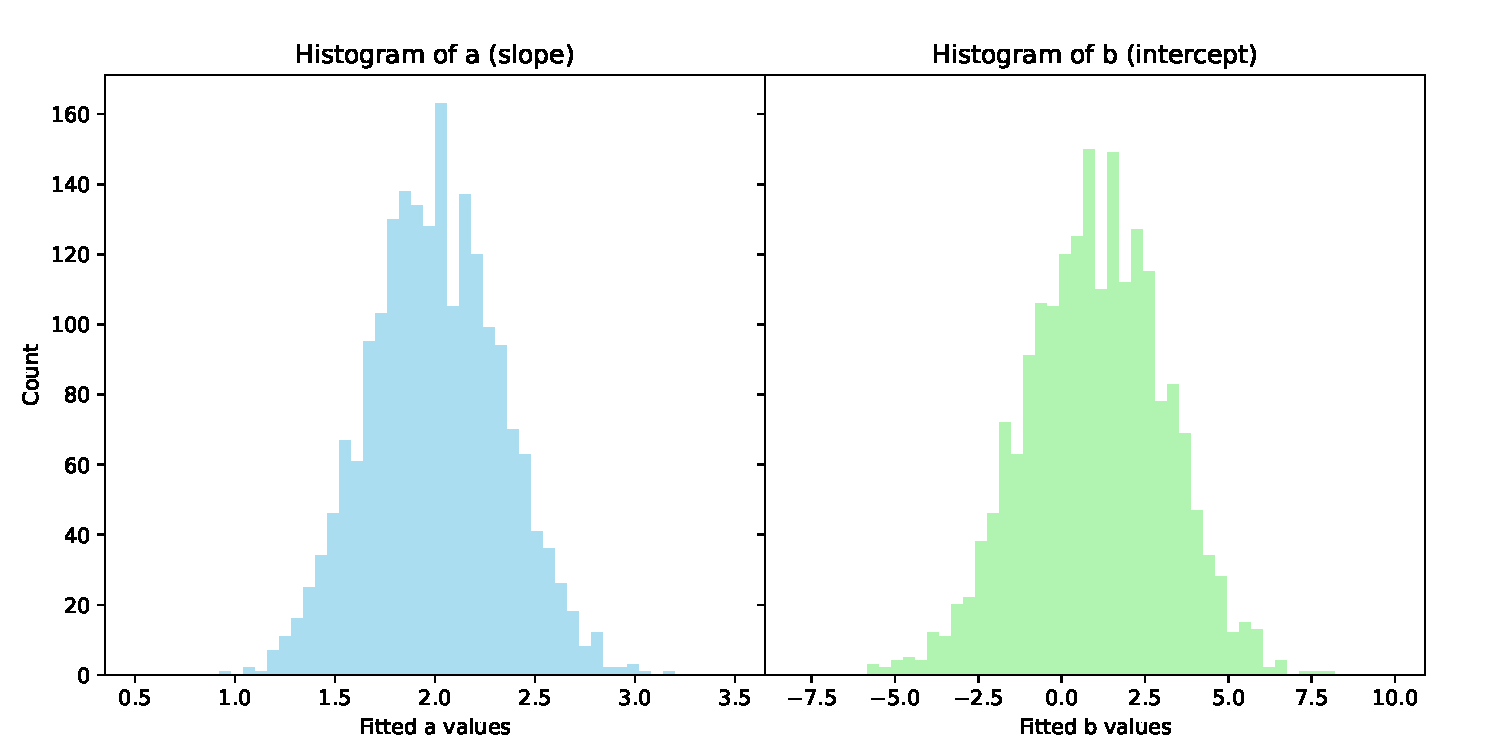
\includegraphics[width=1\linewidth]{figures/output/practice_3/output3_2.pdf}
    \caption{1D Histogram of fitted $a$ and $b$.}
    \label{fig:output_3_2}
\end{figure}

\begin{figure}[h]
    \centering
    \hspace{1cm}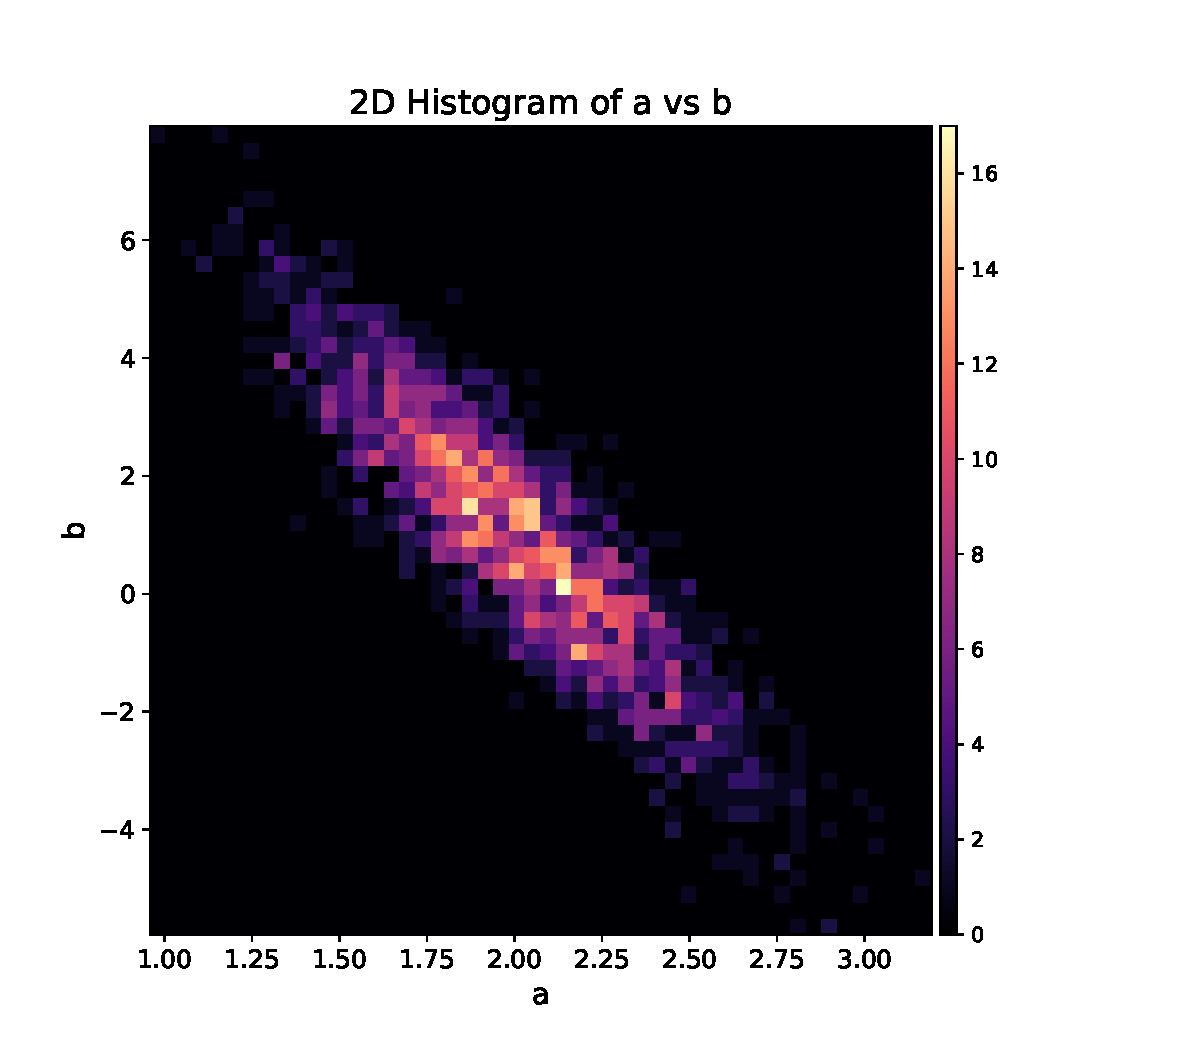
\includegraphics[width=.8\linewidth]{figures/output/practice_3/output3_3.pdf}
    \caption{2D Histogram of fitted $a$ and $b$.}
    \label{fig:output_3_3}
\end{figure}

% \begin{figure}[h]
%     \centering
%     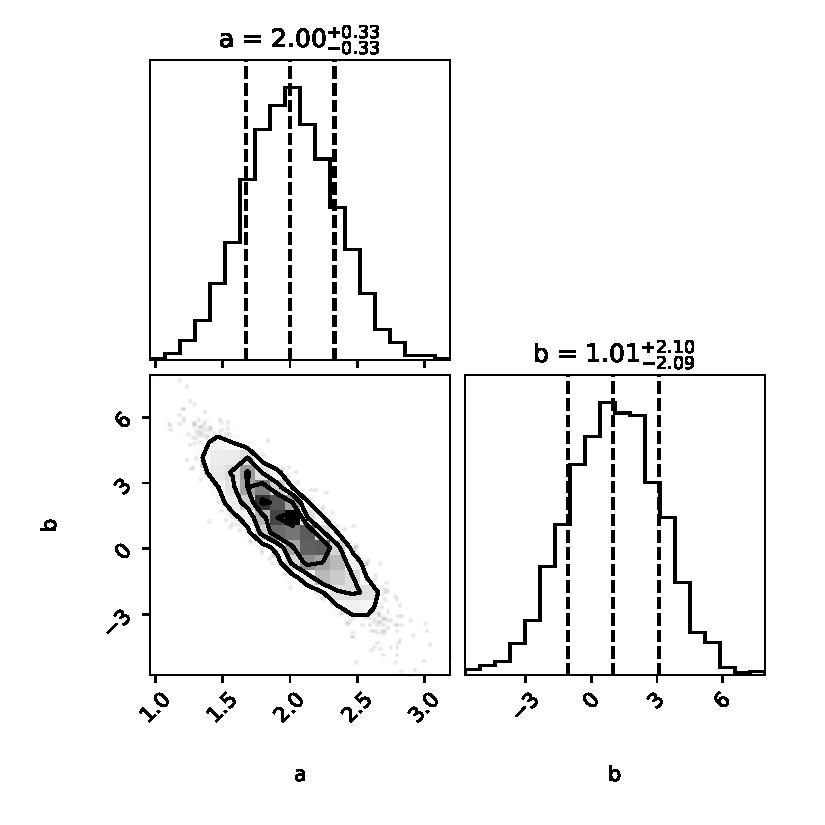
\includegraphics[width=0.5\linewidth]{figures/output/practice_3/output3_3_corner.pdf}
%     \caption{Corner plot of fitted $a$ and $b$}
%     \label{fig:output_3_3_corner}
% \end{figure}
\clearpage

從Fig.\ref{fig:output_3_1}以及Table.\ref{tab:mean_std}可看出資料的標準差$\sigma$大約為3,與原始設定的數值相近,顯示出資料的noise設定是合理的。再使用這10個平均資料點加權線性擬合,以每點的標準差作為權重,可得出結果為$a=2.003$、$b=1.002$,相當接近原始設定值($a=2.0$、$b=1.0$)。

我們將2000組擬合結果的 a 和 b 數值分別繪製成直方圖(Fig.\ref{fig:output_3_2})。可以觀察到 a 的分布大致呈現高斯形態,平均值接近2;b 的分布稍微比較散一點,平均值接近1。此外,從Fig.\ref{fig:output_3_3}的2D直方圖可以看到資料點分佈是一個傾斜的橢圓形,顯示兩數值呈現負相關。即當 a 值增加時, b 會適度減少以確保整理擬合的結果良好,這就是補償效應;a與b的共變異數矩陣以及相關係數矩陣中, $r=-0.893$ 、$R^2=0.797$,也證明了二者之間的強烈負相關性。


% \clearpage
\section{問題討論}
\subsection{Practice 1}\label{subsec:discuss_1}
\hfill

\begin{itemize}
    \item The term \textbf{model} is often used in the statement of goodness of fit. What does \textbf{model} mean in this case?
    \hfill

    Model 在這裡是描述數據在生成時所遵循之機制的數學函數,在本次實驗中,我們令數據從$y=a*x+b$這個基礎下生成數據點,並透過LS\ fitting和$\chi^2$\ fitting來找到擬合參數$a$、$b$。
    
    \item State what \textbf{overfitting} is.\\
    Overfitting(過度擬合)是一種機器學習時出現的不理想行為。Overfitting 發生可能的原因包含模型沒有一般化(資料筆數太少),或是機器學習過程中學到了資料中包含的 noise (模型自由度較高),導致雖然在舊的模型上運作可以得到好的表現,但若是套用到新的數據上,可能會有不好的表現。的時候。因此在將新的數據加入資料集時,overfitting會導致在資料判斷上出錯。在 Practice 1 中以 $y=ax+b+noise$的線性模型產生資料,並加入標準差$σ_0=3$的noise,但因為合理使用線性模型配上線性資料,所以擬合出的結果與理論預期高度一致,沒有觀察到明顯的overfitting情況。

    \item Design an experiment to illustrate the \textbf{overfitting} phenomenon.\\
    To illustrate the overfitting phenomenon, it's crucial to assume a model with a sufficiently large number of parameters to fit our data. In addition, the number of parameters cannot be higher than the data size since the reduced $\chi^2$ ($\chi^2_\nu$ hereafter) is required to evaluate the effectiveness of overfitting quantitatively (According to Eq. \ref{eq:reduced_chi}, $\nu=N-p=0$ makes $\chi^2_\nu$ undefined). In our case, the data size is \texttt{len(x)=10}. The best choice of the model, consequently, is the 8th-degree polynomial, which includes nine free parameters.
    
    \item By making slight adjustments to your code, you can effectively achieve this goal.\\
    We merely modified the \texttt{curve\_fit} section in Fig. \ref{fig:code_1_3} to \texttt{np.polyfit} to fit our data with an 8th-degree polynomial. The fitted coefficients are saved for plotting and reproducing. The reason why we don't continue using \texttt{curve\_fit} is due to simplicity and ignoring the effect of uncertainties.
    \begin{figure}[h]
        \centering
        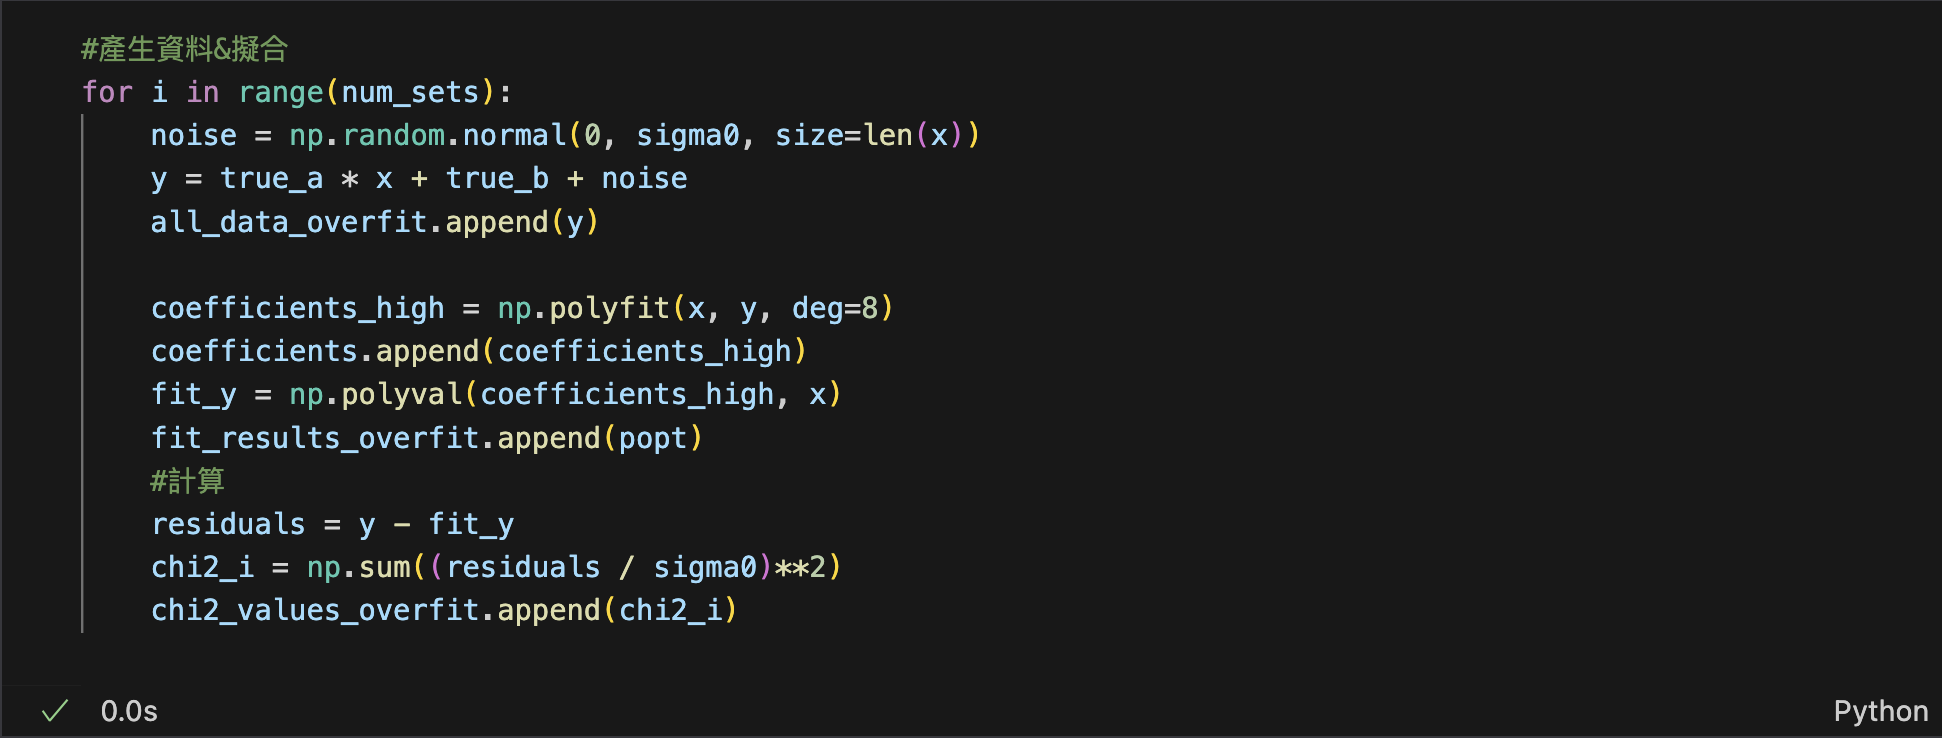
\includegraphics[width=1\linewidth]{figures/code/practice_1/code_1_6.png}
        \caption{Same coding part as Fig. \ref{fig:code_1_4} but the 8th-degree polynomial is used to be the fitting model.}
        \label{fig:code_1_6}
    \end{figure}

    

    % \clearpage
    \item Describe your observations based on the modifications made.\\
    As Fig. \ref{fig:output_1_1_overfit} shows, the fitted curves (green dotted lines) are messier and more complicated than Fig. \ref{fig:output_1_1}. Those curves seem forced to approach the data points, and once the fitted models perform outside the range of the data (the leftmost and rightmost parts of the plot), the curves blow up and down drastically. These phenomena indicate that the models may:
    \begin{itemize}
        \item Fit overly well within the data, minimizing the least-squares significantly.
        \item Fail to extrapolate and predict functionally outside the range of the fitting data, limiting the utility a model means to provide.
    \end{itemize}
    
    \begin{figure}[h]
        \centering
        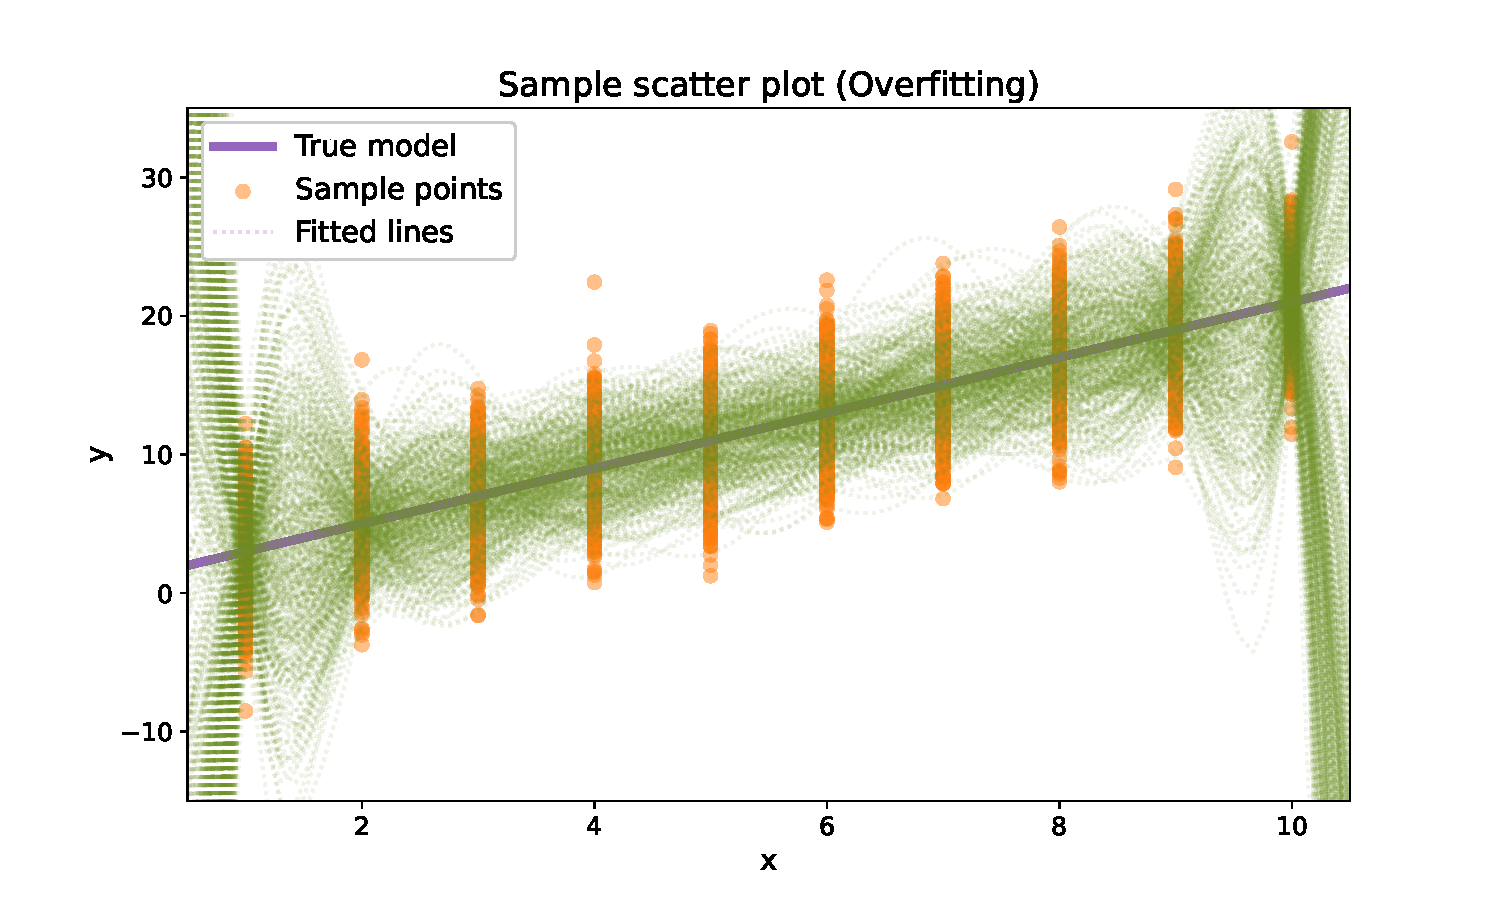
\includegraphics[width=1\linewidth]{figures/output/practice_1/output1_1_overfit.pdf}
        \caption{Same plot as the Fig. \ref{fig:output_1_1} but the fitted lines are 8th-degree polynomials.}
        \label{fig:output_1_1_overfit}
    \end{figure}
    % \begin{figure}[h]
    %     \centering
    %     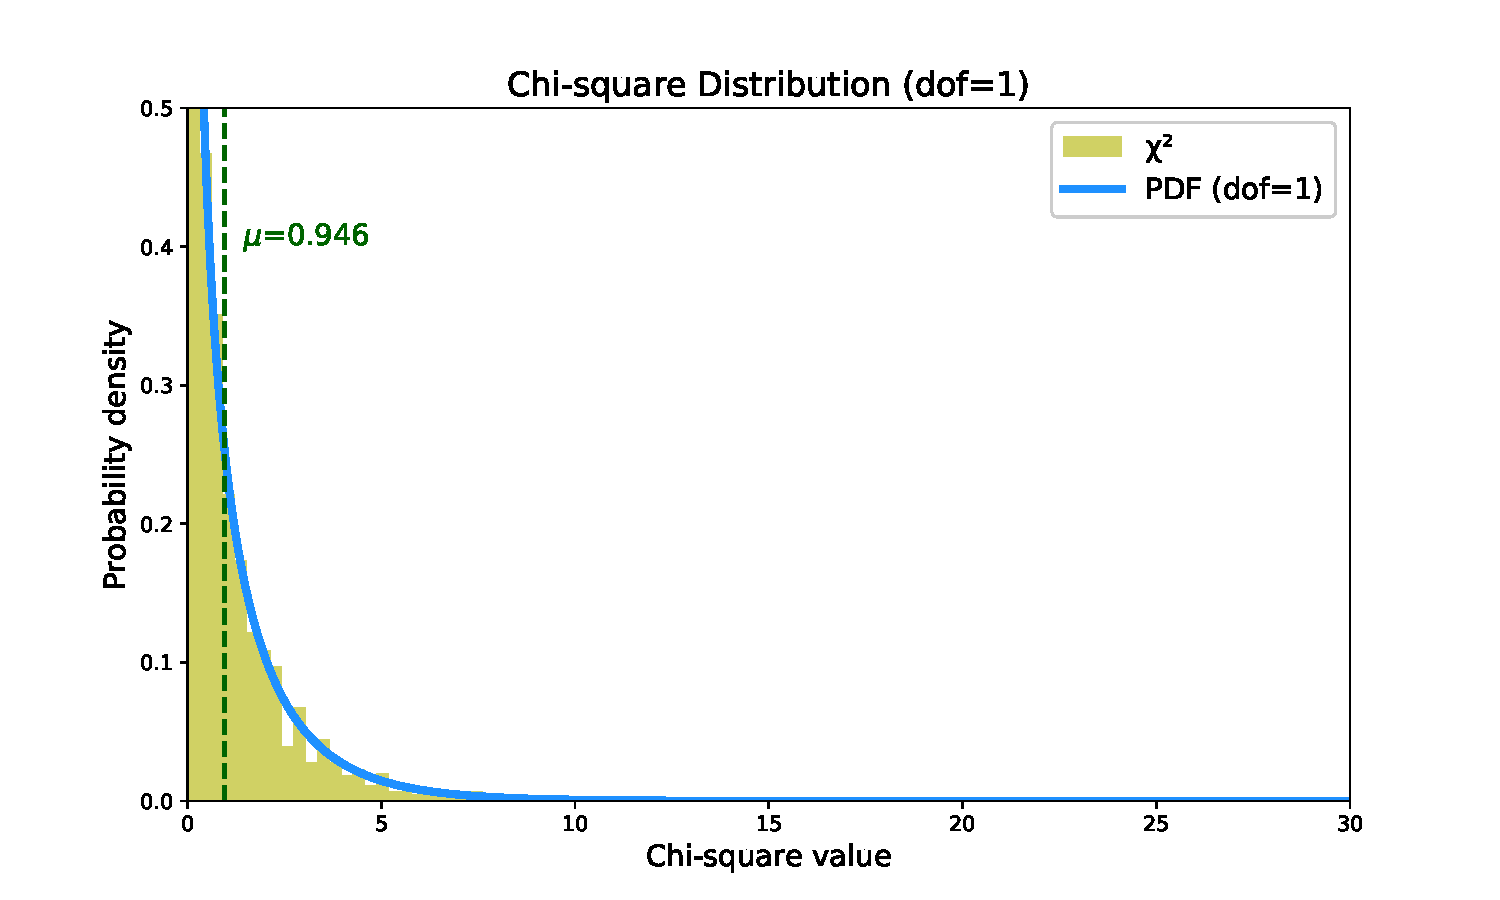
\includegraphics[width=0.8\linewidth]{figures/output/practice_1/output1_2_overfit.pdf}
    %     \caption{Histogram of the chi-square distribution (overfitting)}
    %     \label{fig:output_1_2_overfit}
    % \end{figure}
    The evaluation of $\chi^2_\nu$ can be used to distinguish the difference between the goodness of fit (Sec. \ref{subsec:goodness}). In this case, the just-fitted model is the linear function (Sec. \ref{subsec:result_1}), and the overfitted model is the 8th-degree polynomial. As the two reduced chi-square distributions overlay in Fig. \ref{fig:output_1_2_compare}, several characteristics can be found:
    \begin{itemize}
        \item The shape of the $\chi^2_\nu$ by linear model is compact, and its peak and mean are in the vicinity of the just-fit standard ($\chi^2_\nu=1$), i.e., the linear model may be the just-fitted model.
        \item The distribution of $\chi^2_\nu$ by 8th-degree polynomial (the overfitted model) morphs extremely right-skewed from that of the linear model, suggesting that the vast majority of the 8th-degree polynomials are overfitted to the data points. This is concluded by the fact that the errors are known and assumed, expelling the possibility of overestimation (Sec. \ref{subsec:goodness}).
    \end{itemize}
    \begin{figure}[h]
        \centering
        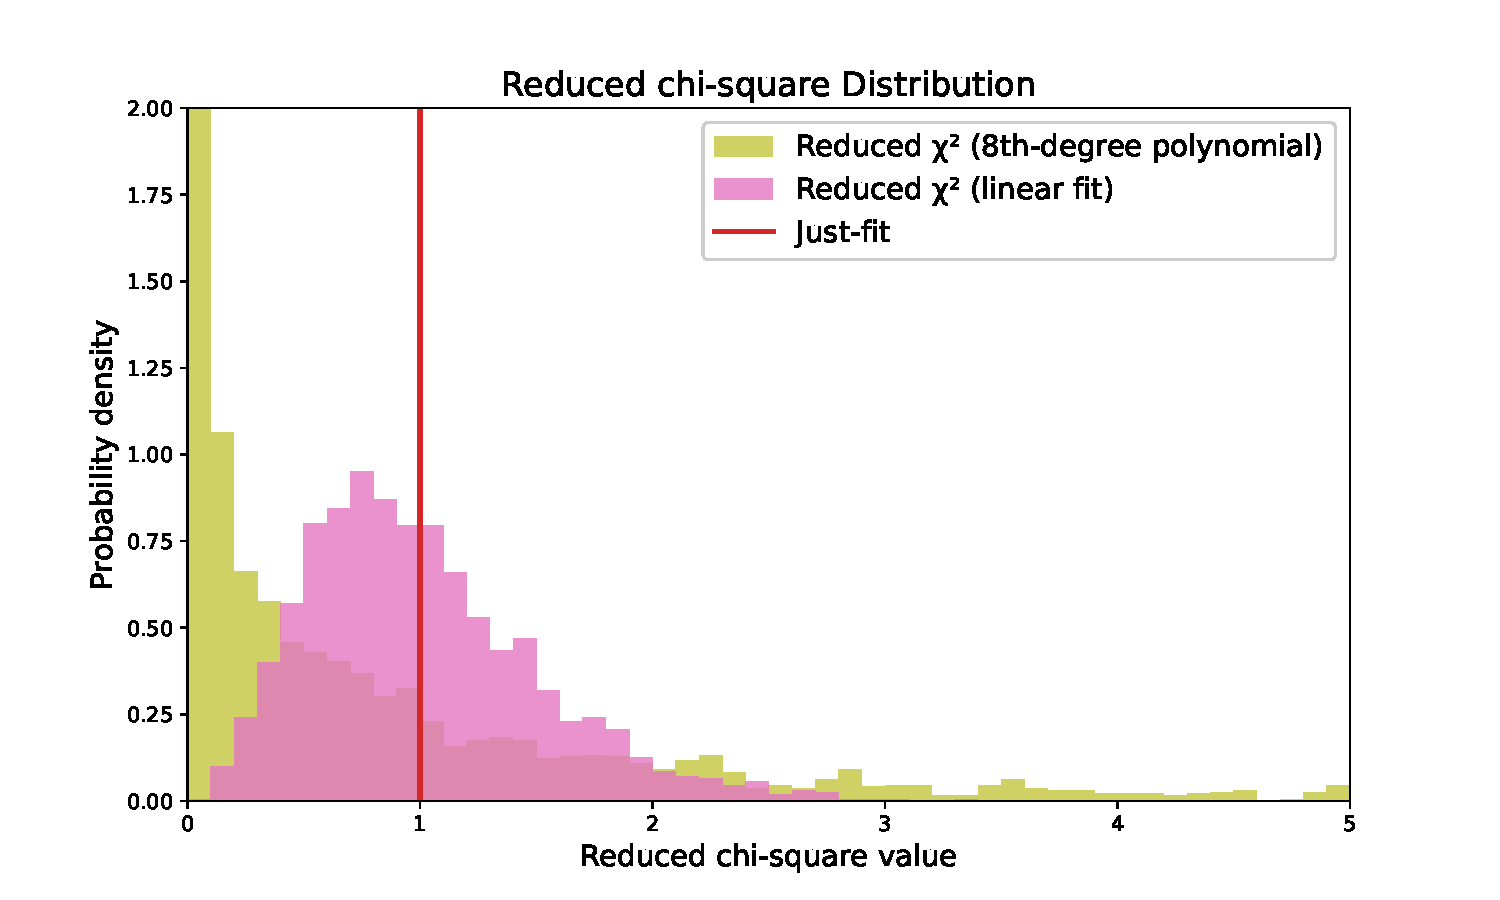
\includegraphics[width=1\linewidth]{figures/output/practice_1/output1_2_hist_compare.pdf}
        \caption{Reduced $\chi^2$ distributions comparison between the two fitting functions, linear functions, and 8th-degree polynomials}
        \label{fig:output_1_2_compare}
    \end{figure}

    \clearpage
    \item Will this phenomenon occur when analyzing the data from the General Physics Laboratory experiments, such as the pendulum or gravity experiment?
    \hfill

    如果我們已經有理論公式(例如單擺實驗公式:$T=2\pi\sqrt\frac{L}{g}$)可讓我們做數據擬合時,過擬合的結果相對不容易出現,因為所選模型是使用物理理論所推論的結果,較不會出現數據擬合到誤差的情況。
    
    
    \item Can we determine if the model is overfitting the data points obtained by unknown functions? Design your own experiment to prove your point of view.\\
    我們可透過\textbf{殘差分析}與\textbf{測試資料的誤差比較}判斷模型是否發生過擬合。
    \begin{enumerate}
        \item 殘差分析:我們可藉由Fig.\ref{fig:residual}看出殘差沒有趨勢,無過擬合或欠擬合的情況發生。
        \begin{figure}[h]
            \centering
            
            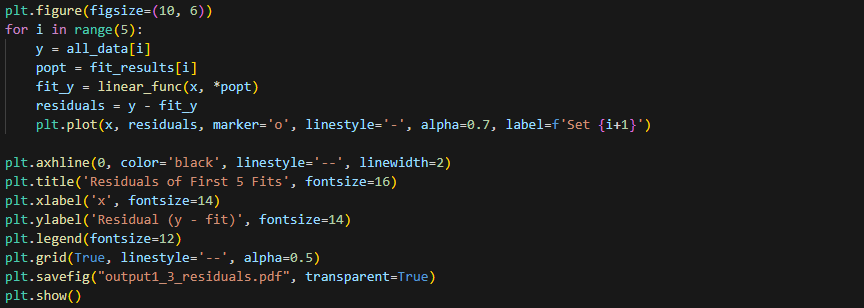
\includegraphics[width=1\linewidth]{figures/code/practice_1/practice 1QA.png}
            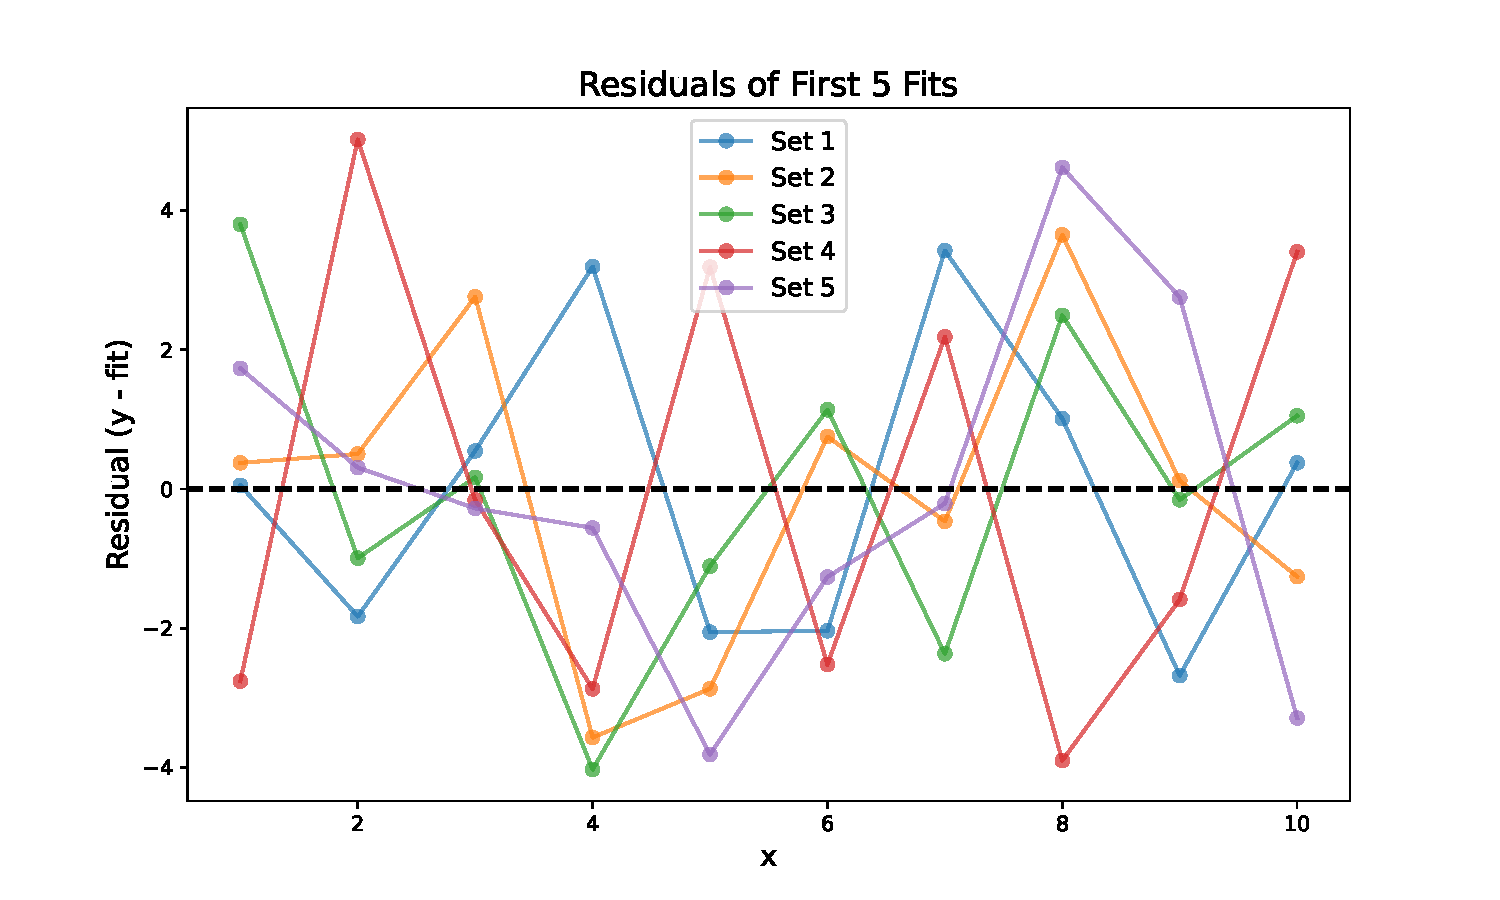
\includegraphics[width=1\linewidth]{figures/output/practice_1/output1_3_residuals.pdf}
            \caption{practice 1之殘插圖程式碼和輸出結果}
            \label{fig:residual}
        \end{figure}
    
        \clearpage
    
        \item 測試資料的誤差比較:透過先產生一組訓練資料,其為一簡單的函數加上雜訊;然後使用不同的model來擬合產生之資料,最後建立一組測試資料來比較模型在未知數據上的誤差;由此可知,當模型在訓練資料上誤差較小、而測試資料上之誤差很大,可說明實驗發生過擬合。
        \begin{figure}[h]
            \centering
            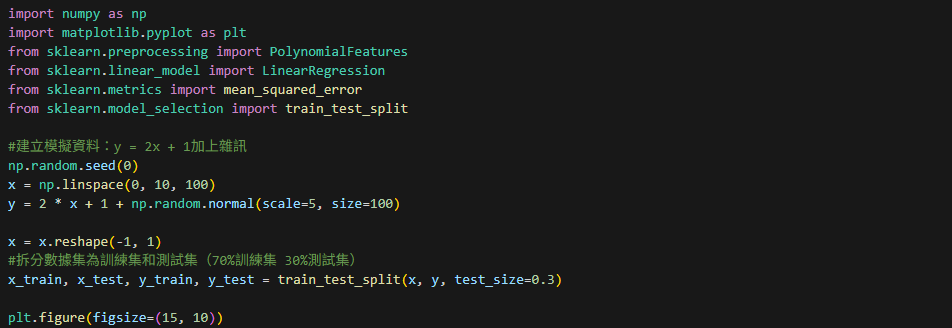
\includegraphics[width=1\linewidth]{figures/code/practice_1/practice_QA2.png}          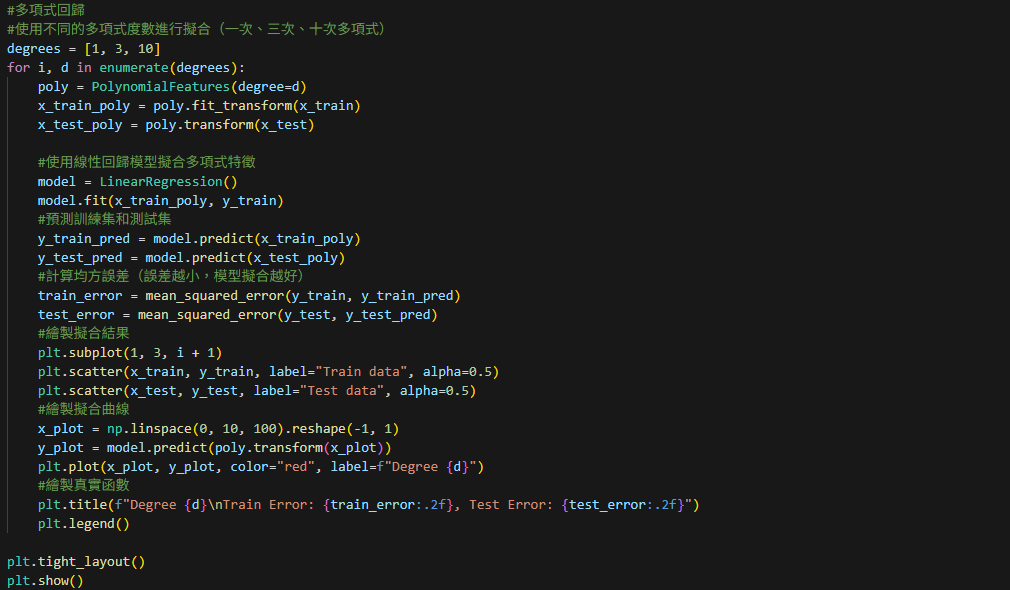
\includegraphics[width=1\linewidth]{figures/code/practice_1/practice_QA3.png}
            \caption{測試資料的誤差比較之程式碼(詳情看註解)}
            \label{fig:practice_design}
        \end{figure}
        
        \clearpage
        
        \begin{figure}[h]
            \centering
            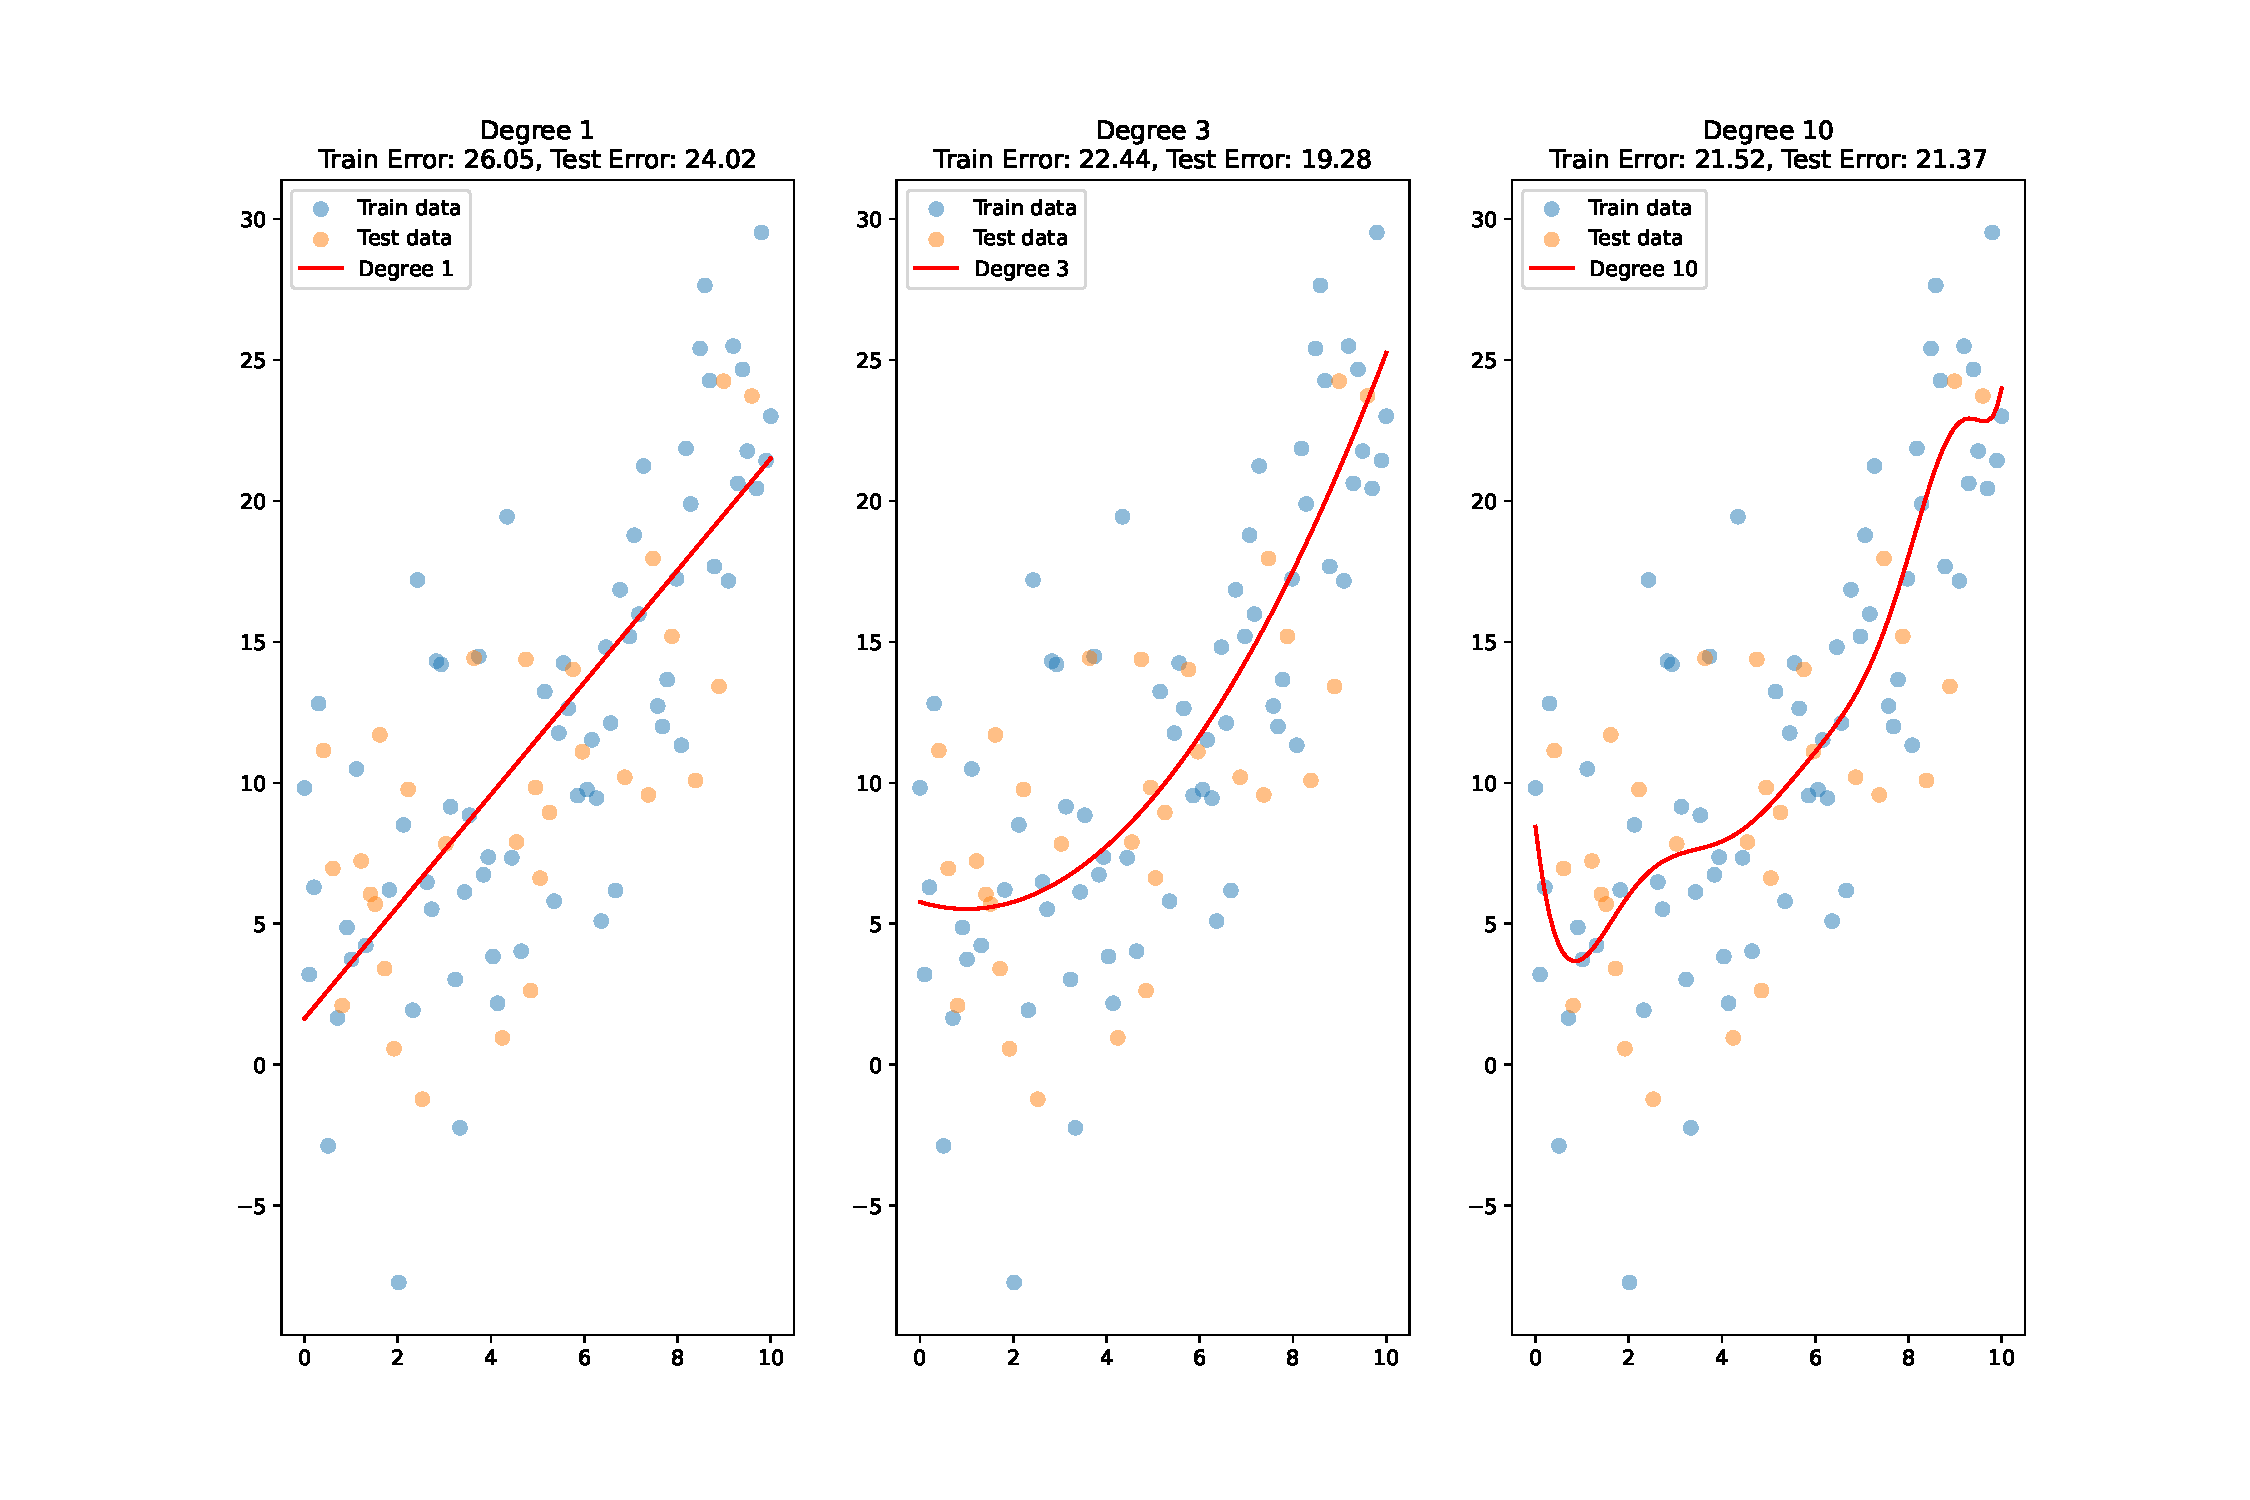
\includegraphics[width=1\linewidth]{figures/output/practice_1/output1_4.pdf}
            \caption{測試資料的誤差比較結果}
            \label{fig:design}
        \end{figure}
        \begin{enumerate}
            \item 使用線性回歸模型(Fig.\ref{fig:design}左圖)
            \begin{itemize}
                \item 訓練誤差為26.05、測試誤差為24.02,可看出單一直線沒辦法更細節的去描繪數據的分布。
                \item 結果:模型過於簡單,發生欠擬合;訓練與測試誤差皆很大。
            \end{itemize}
            \item 使用三次多項式模型(Fig.\ref{fig:design}中圖)
            \begin{itemize}
                \item 訓練誤差為22.44、測試誤差為19.28,模型有畫出資料的趨勢。
                \item 結果:訓練與測試誤差降低,且差距不大,可知結果為good fit。
            \end{itemize}
            \item 使用十次多項式模型(Fig.\ref{fig:design}右圖)
            \begin{itemize}
                \item 訓練誤差為21.52、測試誤差為21.37,模型太過複雜,有許多波動。
                \item 結果:發生過擬合,雖然在訓練誤差是最低的,但測試誤差上升表示訓練誤差所擬合到的是雜訊而不是數據的趨勢。
            \end{itemize}
        \end{enumerate}
    \end{enumerate}
    
\end{itemize}

\clearpage
\subsection{Practice 2}
\hfill

\begin{itemize}
    \item Will $a$ and $b$ be closer to what you originally used to generate the data points in the section with the smaller $\chi^2$ value?\\
    在$\chi^2$值比較小的情況下,a和b會更接近於原始的$a$與$b$的值。這是因為$\chi^2$值小代表資料中的隨機誤差比較小,擬合效果比較好。在$\chi^2$值小的組別中,$a$和$b$的直方圖分布相較於$\chi^2$值大的組別窄、集中,中心值也比較接近真實設定值,資料點與理想直線趨勢接近,誤差小,較能忠實反映真實趨勢。因此使用χ² 值比較小的數據就能得出較不受誤差干擾、類似於原始數據的數值。

    \item Is it appropriate to assess the goodness of fit based solely on the accuracy of the fitted $a$ and $b$ values?\\
    Goodness of fit應以統計方法為主,僅依賴擬合參數的數值準確度可能會產生極大誤差。因為參數數值接近真實值也不代表整體的擬合情況好,如果資料的殘差分佈不符合模型假設,像是有系統誤差或者非高斯noise,整體擬合結果可能會是不好的。且單從參數值會無法看出部分問題,像次資料如果系統性的偏移或異常點,就會產生問題。而且在實際應用中,有可能會不知道真正的$a$和$b$的值,所以也無法單純靠比對參數來評估擬合好壞。從Practice 2的結果也可以看出,即使部分的$a$和$b$的數值接近真實值,但資料隨機誤差較大的區段擬合的不確定性依然很高,分布也會明顯變寬,因此最好還是根據統計量來評估(像是$\chi^2$值、殘差分析或是p-value),在不知道真實參數的時候也還是能分辨出模型是否合理。
\end{itemize}


% \clearpage
\subsection{Practice 3}
\hfill

\begin{itemize}
    \item Explain how you calculate the correlation coefficient from $a$ and $b$ values.

    在本次實驗中,我們用了以下三種方法來計算a和b之correlation coefficient:
    \begin{enumerate}
        \item 使用共變異數矩陣計算:\\我們從\texttt{curve\_fit}函數中獲得之covarianve matrix為:
        \begin{equation}
            covarianve\ martix=\left[
            \begin{array}{cc}
                 \sigma_a^2&cov(a,\ b)  \\
                 cov(b,\ a)&\sigma_b^2 
            \end{array}
            \right]\approx\left[
            \begin{array}{cc}
                 0.110&-0.620  \\
                 -0.620&4.375 
            \end{array}
            \right]
            \nonumber
        \end{equation}
        而根據相關係數之定義:
        \begin{equation}
            R=\frac{cov(a,\ b)}{\sigma_a\sigma_b}
            \nonumber
        \end{equation}
        帶入數值:
        \begin{equation}
            R=\frac{-0.620}{\sqrt{0.110}\cdot \sqrt{4.375}}\approx-0.893
            \nonumber
        \end{equation}
        \item 使用\texttt{numpy.corrcoef()}:\\透過計算所有a、b值之相關係數矩陣再度確認兩者具高度負相關。
        \begin{equation}
            covarianve\ martix=\left[
            \begin{array}{cc}
                 1&-0.893  \\
                 -0.893&1 
            \end{array}
            \right]
            \nonumber
        \end{equation}
        \clearpage
        其中矩陣內各數字表示:
       \begin{table}[h]
    \centering
    \begin{tabular}{|c|c|c|}
        \hline
        位置 & 數學式 & 意義 \\
        \hline
        $[0, 0]$ & $\mathrm{corr}(a, a) = 1$ & $a$與自己的相關係數(恆為1) \\
        \hline
        $[0, 1]$ & $\mathrm{corr}(a, b) = r$ & $a$與$b$之相關係數(我們欲求之) \\
        \hline
        $[1, 0]$ & $\mathrm{corr}(b, a) = r$ & $b$與$a$之相關係數(和 $[0, 1]$ 相同) \\
        \hline
        $[1, 1]$ & $\mathrm{corr}(b, b) = 1$ & $b$與自己的相關係數(恆為1) \\
        \hline
    \end{tabular}
    \caption{相關係數矩陣中各元素的意義}
    \label{tab:corr_matrix}
\end{table}
        \item 利用線性回歸分析\textbf{$b=m\cdot a+c$}:\\我們將a、b視為二維資料點做線性回歸,所得斜率為$-5.624$、截距為$12.242$、相關係數$r=-0.893$,$R^2=0.797$表示約有$79.7\%$之變異可藉由線性關係解釋。
    \end{enumerate}
    此三種方式皆表示a和b之間存在負線性關係,這結果與Fig.\ref{fig:output_3_3}之2D直方圖之結果相符。
\end{itemize}



%%%%%%%%%%%%%%%%

\section{總結}
\hfill

本實驗再次以數值模擬方式,深入探討線性曲線的擬合過程,並對於擬合中的擬合參數a與b與$\chi^2$ distribution的關係,以及透過設計實驗,觀察並了解overfitting的發生和造成的結果。 Practice 1裡,我們建立了產生資料、擬合資料、以及卡方計算等等的基本流程,並驗證了 $\chi^2$ 值符合理論的$\chi^2$ distribution,確定了擬合結果良好。Practice 2 中,我們依照 $\chi^2$ 值的大小將資料分群,並透過分群發現了擁有較小 $\chi^2$ 數值的組別,參數(a與b)的分佈皆較擁有較大 $\chi^2$ 數值的組別集中,數值比較接近真實值,而$\chi^2$ 數值較大的組別則會看出參數分布更加發散、偏移。Practice 3 中以統計方法計算參數的平均值、標準差、共變異數與相關係數,再以 2D 分佈圖與線性回歸驗證在直線擬合中, a的增加會使 b 需要相應地減小, a 與 b 的相關係數約為$-0.963$,呈高度負相關。我們也做了線性回歸分析,得到負斜率回歸線,明確證明了兩者間的負向線性關係。在 overfitting 的探討實驗中,我們以8次多項式擬合小量資料,觀察到擬合曲線在資料範圍外劇烈擺動,以及 reduced $\chi^2$ 分布右偏、拉長等特徵,驗證高自由度的模型在資料有限時容易過度擬合的問題。
本實驗再次深化了我們對曲線擬合的理解,也為將來實驗分析提供實用的統計與實作方法。



\section{分工}
\begin{itemize}
    \item 洪瑜: 實驗分析、問題討論
    \item 黃巧涵: 實驗分析、問題討論
    \item 洪懌平: 實驗分析、問題討論
\end{itemize}


% \clearpage
\section{Appendix}

\subsection{Source code}

\begin{itemize}
    \item \url{https://github.com/hyp0515/exp_phy_ii/tree/main/may6}
\end{itemize}

%--------------------------------------------------------------%
\end{CJK}
\end{document}